% mnras_template.tex 
%
% LaTeX template for creating an MNRAS paper
%
% v3.0 released 14 May 2015
% (version numbers match those of mnras.cls)
%
% Copyright (C) Royal Astronomical Society 2015
% Authors:
% Keith T. Smith (Royal Astronomical Society)

% Change log
%
% v3.0 May 2015
%    Renamed to match the new package name
%    Version number matches mnras.cls
%    A few minor tweaks to wording
% v1.0 September 2013
%    Beta testing only - never publicly released
%    First version: a simple (ish) template for creating an MNRAS paper

%%%%%%%%%%%%%%%%%%%%%%%%%%%%%%%%%%%%%%%%%%%%%%%%%%
% Basic setup. Most papers should leave these options alone.
\documentclass[fleqn,usenatbib]{mnras}

% MNRAS is set in Times font. If you don't have this installed (most LaTeX
% installations will be fine) or prefer the old Computer Modern fonts, comment
% out the following line
\usepackage{newtxtext,newtxmath}
\usepackage{stfloats}
\usepackage[flushleft]{threeparttable}
% Depending on your LaTeX fonts installation, you might get better results with one of these:
%\usepackage{mathptmx}
%\usepackage{txfonts}

% Use vector fonts, so it zooms properly in on-screen viewing software
% Don't change these lines unless you know what you are doing
\usepackage[T1]{fontenc}
\usepackage{setspace}

% Allow "Thomas van Noord" and "Simon de Laguarde" and alike to be sorted by "N" and "L" etc. in the bibliography.
% Write the name in the bibliography as "\VAN{Noord}{Van}{van} Noord, Thomas"
%\DeclareRobustCommand{\VAN}[3]{#2}
%\let\VANthebibliography\thebibliography
%\def\thebibliography{\DeclareRobustCommand{\VAN}[3]{##3}\VANthebibliography}


%%%%% AUTHORS - PLACE YOUR OWN PACKAGES HERE %%%%%

% Only include extra packages if you really need them. Common packages are:
\usepackage{graphicx}	% Including figure files
\usepackage{amsmath}	% Advanced maths commands
\let\Bbbk\relax
\usepackage{amssymb}	% Extra maths symbols
\usepackage[justification=centering]{caption}
\usepackage{float}
%% Reintroduced the \received and \accepted commands from AASTeX v5.2
%\received{June 1, 2019}
%\revised{January 10, 2019}
%\accepted{\today}
%% Command to document which AAS Journal the manuscript was submitted to.
%% Adds "Submitted to " the argument.

%\title[Short title, max. 45 characters]{Periodic X-ray Sources in the Galactic Bulge}
%\author{Bao \& Li}

\title[Periodic X-ray Sources in the Galactic Bulge]{Periodic X-ray Sources in the Galactic Bulge: Application of the Gregory-Loredo Algorithm}

\author[Bao \& Li]{
Tong Bao,$^{1,2}$\thanks{E-mail: baotong@smail.nju.edu.cn}
Zhiyuan Li,$^{1,2}$\thanks{E-mail: lizy@nju.edu.cn}
\\
% List of institutions
$^{1}$School of Astronomy and Space Science, Nanjing University, Nanjing 210046, China\\
$^{2}$Key Laboratory of Modern Astronomy and Astrophysics (Nanjing University), Ministry of Education, Nanjing 210046, China
}

% These dates will be filled out by the publisher
\date{Accepted XXX. Received YYY; in original form ZZZ}

% Enter the current year, for the copyright statements etc.
\pubyear{2015}

\begin{document}
\maketitle
%\correspondingauthor{August Muench}
%\email{greg.schwarz@aas.org, gus.muench@aas.org}
\begin{abstract}
We present the discovery of 23 X-ray periodic sources in the Limiting Window (LW), a low-extinction region in the Galactic bulge, locating 80' south of the Galactic center. Their luminosities range(${\rm 10^{31}-10^{33} ~erg ~ s^{-1}}$) and period distribution(mostly between 1 to 3 hour), indicate they are cataclysmic variables (CVs). Most of them are polars with relatively harder spectrum, suggesting an unusual sub-class of mCVs.
The brighter sources (6 out of 23 with L>$\rm 10^{32} ~erg~s^{-1}$) in this sample are more likely IPs, with mean $M_{WD}$ about 0.8 $M_\odot$.
We also proved that the Gregory-Loredo (GL) method used in this work has better sensitivity and data usage compared to the Lomb-Scargle (LS) method. In combination with the simulation and the geometry of accretion in CVs, we constrain the proportion of polars to X-ray sources in LW about 17\%, and the fraction of DNe is about 25\%, though with more uncertainty. Still, this discovery confirms the sub-type of unusual mCVs and provides a practical way to study the population about X-ray sources based on periodic modulation.
\end{abstract}

%% Keywords should appear after the \end{abstract} command. 
%% See the online documentation for the full list of available subject
%% keywords and the rules for their use.
%\keywords{Galaxy: bulge --- X-rays: stars --- X-rays: binaries}
\begin{keywords}
Galaxy: bulge --- X-rays: stars --- X-rays: binaries
\end{keywords}

\section{Introduction} \label{sec:intro}
X-ray-emitting, close binaries, which involve an black hole, a neutron star or a white dwarf (WD) accreting from a companion star, are among the first objects discovered in the X-ray sky and now understood to be ubiquitous in the local universe. As such, X-ray binaries can serve as a useful probe of their parent stellar populations.
In particular, cCataclysmic variables (CVs), are close binary including a white dwarf (WD) and a main-sequence or sub-giant companion, whose material could be accreted by Roche-lobe overflow or stellar wind. 
They can be divided into magnetic (mCVs) and nonmagnetic CVs (non-mCVs) according to their magnetic field strengths of WDs. In addition, the mCVs are split into polars ($P_{spin}/P_{orb}\simeq 1$) and IPs ($P_{spin}/P_{orb}\simeq 0.01-1$), depending on their level of synchronization. 
The evolution of CVs are driven by angular momentum losses (AML) to keep the period from expanding, which would made system detached. The existence of  "period gap" is caused by the change of mechanism for angular momentum losses.  The dominant AML mechanism in long-period
systems ($P_{orb}$ $\geq$ 3 hour) is "magnetic braking", whereas short-period CVs ($P_{orb}$ $\leq$ 2 hour) are  driven by gravitational radiation. Meanwhile, there is a minimum period of CVs, resulted from the mass-loss-induced loss of thermal equilibrium in companion star. The orbital period of CVs are mainly between 1 to 10 hours, making it suitable for X-ray timing analysis. 

It has been proved that the collective properties of CVs serve as great probe for dynamic interactions of their local environment, contributed from the high abundance of WDs in binaries. The effect would be remarkable only with extremely high stellar density (e.g. galactic center or global clusters \citep{2019ApJ...876...59C}) for us obtaining observable evidence in Hubble time. 
In addition to that, the individual properties of CVs provide hints for the accretion region and magnetic field, especially from their periodic variability.

It has been suggested that the thousands of X-ray sources in galactic center are magnetic cataclysmic variables, particularly intermediate
polars (IPs) \citep{2009ApJS..181..110M,2018ApJS..235...26Z}. Due to the lack of optical/infrared imaging and spectroscopy resulted from high extinction and source crowding, the direct identification of them has been really difficult.
In fact, even the presence and characteristics of the He II $\lambda 4686$ and H$\beta$ line have been often used to judge if a CV is magnetic or not, the proof is far from conclusive. In \cite{1992PhDT.......119S}, many IPs with weak H$\beta$ lines could not be identified from non-magnetic systems using this diagnostic. 
Hence the periodicity becomes a well recognized probe to study their population, because of their different features in periodic modulation (see Section~\ref{subsec:class}).  

In \citet{2003ApJ...599..465M}, eight periodic sources were identified as mCVs in galactic center region (GCR). Then for galactic bulge region, ten periodic sources were found by using Lomb-Scargle methods \citep{2012ApJ...746..165H}. They were believed as an unusual type of mCVs with harder spectra like IPs while their period distribution resembles that of polars. The research was based on the observation of low-extinction Window fields (LW), locating at $1^{\circ}4$ south of the Galactic center. Its rarity of avoiding the obscuration from molecular cloud deserved our deeper excavation of these X-ray sources. 
Besides, according to RK catalog \citep{2003A&A...404..301R}, the mCVs (mostly DNe) occupied 20\% in CVs sample, while for GCR, this fraction was reckoned over 30-40\% \citep{2016ApJ...826..160H,2012ApJ...746..165H}. The miss of non-mCVs demands reliable explanation from analyzing the properties of these sources. It may indicates that a large number of non-mCVs still awaits discovery since faint class can be always missed in flux-limited surveys.

In this work, we revisit the {\it Chandra} observations of the LW, employing a novel technique, known as the Gregory-Loredo period searching algorithm, to detect periodic signals in the LW. Meanwhile, the methods with more efficiency and the simulation with higher accuracy have been both operated. 
We explored the X-ray properties of 23 periodic sources (ten of them identified in \cite{2012ApJ...746..165H}). 
In Section~\ref{sec:obs}, we describe the preparation of the X-ray data and a raw list of X-ray sources in the LW.
We then provide in Section~\ref{sec:methods} a brief overview of the period searching methods, with an emphasis on the Gregory-Loredo algorithm.main methods for period finding and focuses on the GL method we adopted in this work. 
Section~\ref{sec:results} is devoted to the period searching results.
Section~\ref{sec:spectra} presents an X-ray spectral analysis for the detected periodic sources. 
The comparison with previous work, the identification for these periodic sources and the X-ray source population in the LW would be discussed in Section~\ref{sec:discussion}.
A summary of this study is given in Section~\ref{sec:summary}.

\section{X-ray Data Preparation} \label{sec:obs}
\subsection{{\it Chandra} observations} \label{subsec:xdata}
The LW towards the inner Galactic bulge has been extensively observed by {\it Chandra} with its Advanced CCD Imaging Spectrometer (ACIS).
A total of 13 ACIS-I observations were taken, three in 2005 and ten in 2008, resulting in a total exposure of 982 ks.
A log of these observations is given in Table \ref{tab:obsinfo}. 
A number of previous studies have made use of all or part of these observations, which primarily focused on the identification of discrete X-ray sources and the quantification of their statistical properties \citep{2009Natur.458.1142R,2009ApJ...700.1702V,2009ApJ...706..223H,2011MNRAS.414..495R,2012MNRAS.427.1633H,2013ApJ...766...14M,2016MNRAS.462L.106W}.

%\decimalcolnumbers
\begin{table*}
\centering
\caption{{\it Chandra} observations of the Limiting Window} \label{tab:obsinfo}
\centering
\begin{tabular}{ccccccc}
\hline
\hline
ObsID & Start Time & Nominal R.A. & Nominal Decl. &  Roll angle & Exposure & Mode\\
& UT & ($\circ$) & ($\circ$) & ($\circ$) & ks & \\ 
\hline
6362 & 2005-08-19 16:15 & 267.86875 & -29.58800 & 273 & 37.7 & FAINT \\
5934 & 2005-08-22 08:16 & 267.86875 & -29.58800 & 273 & 40.5 & FAINT \\
6365 & 2005-10-25 14:55 & 267.86875 & -29.58800 & 265 & 20.7 & FAINT \\
9505 & 2008-05-07 15:29 & 267.86375 & -29.58475 & 82  & 10.7 & VFAINT \\
9855 & 2008-05-08 05:00 & 267.86375 & -29.58475 & 82  & 55.9 & VFAINT \\
9502 & 2008-07-17 15:45 & 267.86375 & -29.58475 & 281 & 164.1 & VFAINT \\
9500 & 2008-07-20 08:11 & 267.86375 & -29.58475 & 280 & 162.6 & VFAINT \\
9501 & 2008-07-23 08:13 & 267.86375 & -29.58475 & 279 & 131.0 & VFAINT \\
9854 & 2008-07-27 05:53 & 267.86375 & -29.58475 & 278 & 22.8 & VFAINT \\
9503 & 2008-07-28 17:37 & 267.86375 & -29.58475 & 275 & 102.3 & VFAINT \\
9892 & 2008-07-31 08:07 & 267.86375 & -29.58475 & 275 & 65.8 & VFAINT \\
9893 & 2008-08-01 02:44 & 267.86375 & -29.58475 & 275 & 42.2 & VFAINT \\
9504 & 2008-08-02 21:23 & 267.86375 & -29.58475 & 275 & 125.4 & VFAINT \\
\hline
\end{tabular}
\end{table*}

We downloaded and uniformly reprocessed the archival data with CIAO v4.10 and CALDB v4.8.1, following the standard procedure\footnote{http://cxc.harvard.edu/ciao}.
The CIAO tool \emph{reproject\_aspect} was employed to align the relative astrometry among the individual observations, by matching the centroids of commonly detected point sources. ObsID 9502, which has the longest exposure (164.1 ks), served as the reference frame.
%The resultant accuracy in relative astrometry was typically better than $0\farcs1$.
The level 2 event file was created for each ObsID, with the arrival time of each event corrected to the Solar System barycenter (i.e., Temps Dynamique Barycentrique time) by using the CIAO tool \emph{axbary}.
We then constructed a merged event list, reprojecting all events to a common tangential point, [R.A., Decl.]=[267.86375, 29.58475].
The individual observations cover a similar field-of-view (FoV) due to their similar aimpoints and roll angles, as illustrated in Figure~\ref{fig:FoV} which displays the merged 2--8 keV counts image.
We have examined the light curve of each ObsID and found that the instrumental background was quiescent for the vast majority of time intervals.
Hence we preserved all the science exposures for source detection and subsequent timing analysis, taking the advantage of uninterrupted signals within each observation.  

\subsection{Source detection}\label{subsec:detect}
It is known that the LW suffers from moderate line-of-sight extinction, $N_{\rm H} \approx 7\times10^{21}{\rm~cm^{-2}}$ \citep{2011MNRAS.414..495R}, which obscures X-ray photons with energies $\lesssim$ 1 keV.
%there would be a large number of active binaries (AB) as foreground sources. ABs emit X-rays mainly below 2keV. Thus we use 2-8 keV to do source detection. 
Here we focus on sources prominent in the 2--8 keV band, which are most likely CVs located in the Galactic bulge. This will also facilitate a direct comparison with the CVs found in the Nuclear Star Cluster \citep{2018ApJS..235...26Z}, the line-of-sight column density of which, $N_{\rm H} \sim 10^{23}{\rm~cm^{-2}}$, is only transparent to photons with energies $\gtrsim$2 keV. 

Source detection was performed following the procedures detailed in \citet{2018ApJS..235...26Z}.
Briefly, we first generated for each observation an exposure map as well as point-spread function (PSF) maps with enclosed count fraction (ECF) of 50\% and 90\%. 
Both the exposure and PSF maps were weighted by a fiducial spectrum, which is an absorbed bremsstrahlung with a plasma temperature of 10 keV and a column density of $N_{\rm H}=10^{22}{\rm~cm^{-2}}$, representative of the X-ray sources in the LW. 
We then reprojected the individual exposure maps to form a stacked exposure map in the same way as for the counts images; the PSF maps were similarly stacked, weighted by the corresponding exposure map. 
Next, we employed {\it wavdetect} to identify discrete sources in the merged 2--8 keV counts image, supplying the algorithm with the stacked exposure map and the 50\%-ECF PSF map and adopting a false-positive probability threshold of $10^{-6}$. 
This resulted in a raw list of 847 independent sources in the 2--8 keV band. 
% {\bf [since photometry is involved in the timing anlysis, it's not a bad idea to describe the procedure here]}
%Since the goal of this paper is to identity periodic sources and we can only get robust periodic signal from relatively bright sources. The precise photometry correction for these sources are not necessary.

The source centroid derived from {\it wavdetect} was refined using a maximum likelihood method that iterates over the detected counts within the 90\% enclosed counts radius (ECR).
Starting from this step we consider the 1--8 keV band to maximize the signal from potential sources in the LW. 
Then, for each ObsID, source counts were extracted from the 90\% ECR, while background counts were extracted from a concentric annulus with inner-to-outer radii of 2--4 times the 90\% ECR, excluding any pixel falling within 2 times the 90\% ECR of neighboring sources.
Source crowding is not a general concern in the LW, but in a few cases the source extraction region was reduced to 50\% ECR due to otherwise overlapping sources. 
The total source and background counts were obtained by summing up the individual observations. 
Photometry (i.e., net photon flux and its error) for individual sources were calculated using the CIAO tool \emph{aprates}, which takes into account the local effective exposure, background and ECF. 
We consider a {\it significant detection} for a given source in a given ObsID if the photon flux is greater than 3 times the error. 
%For precisely processing, we exclude the contamination of nearby point sources and extended sources from background region by naked eyes. 
%Then this procedure was only applied for candidate periodic sources (as decribed in sec \ref{sec:results}) due to the manpower limit. 
We further define for each source an inter-observation {\it variability index}, $\rm VI=S_{max}/S_{min}$, where $\rm S_{max}$ and $\rm S_{min}$ are the maximum and minimum photon fluxes among all the significant detections, respectively. This implicitly requires significant detections in at least two observations.

\begin{figure*}
\centering
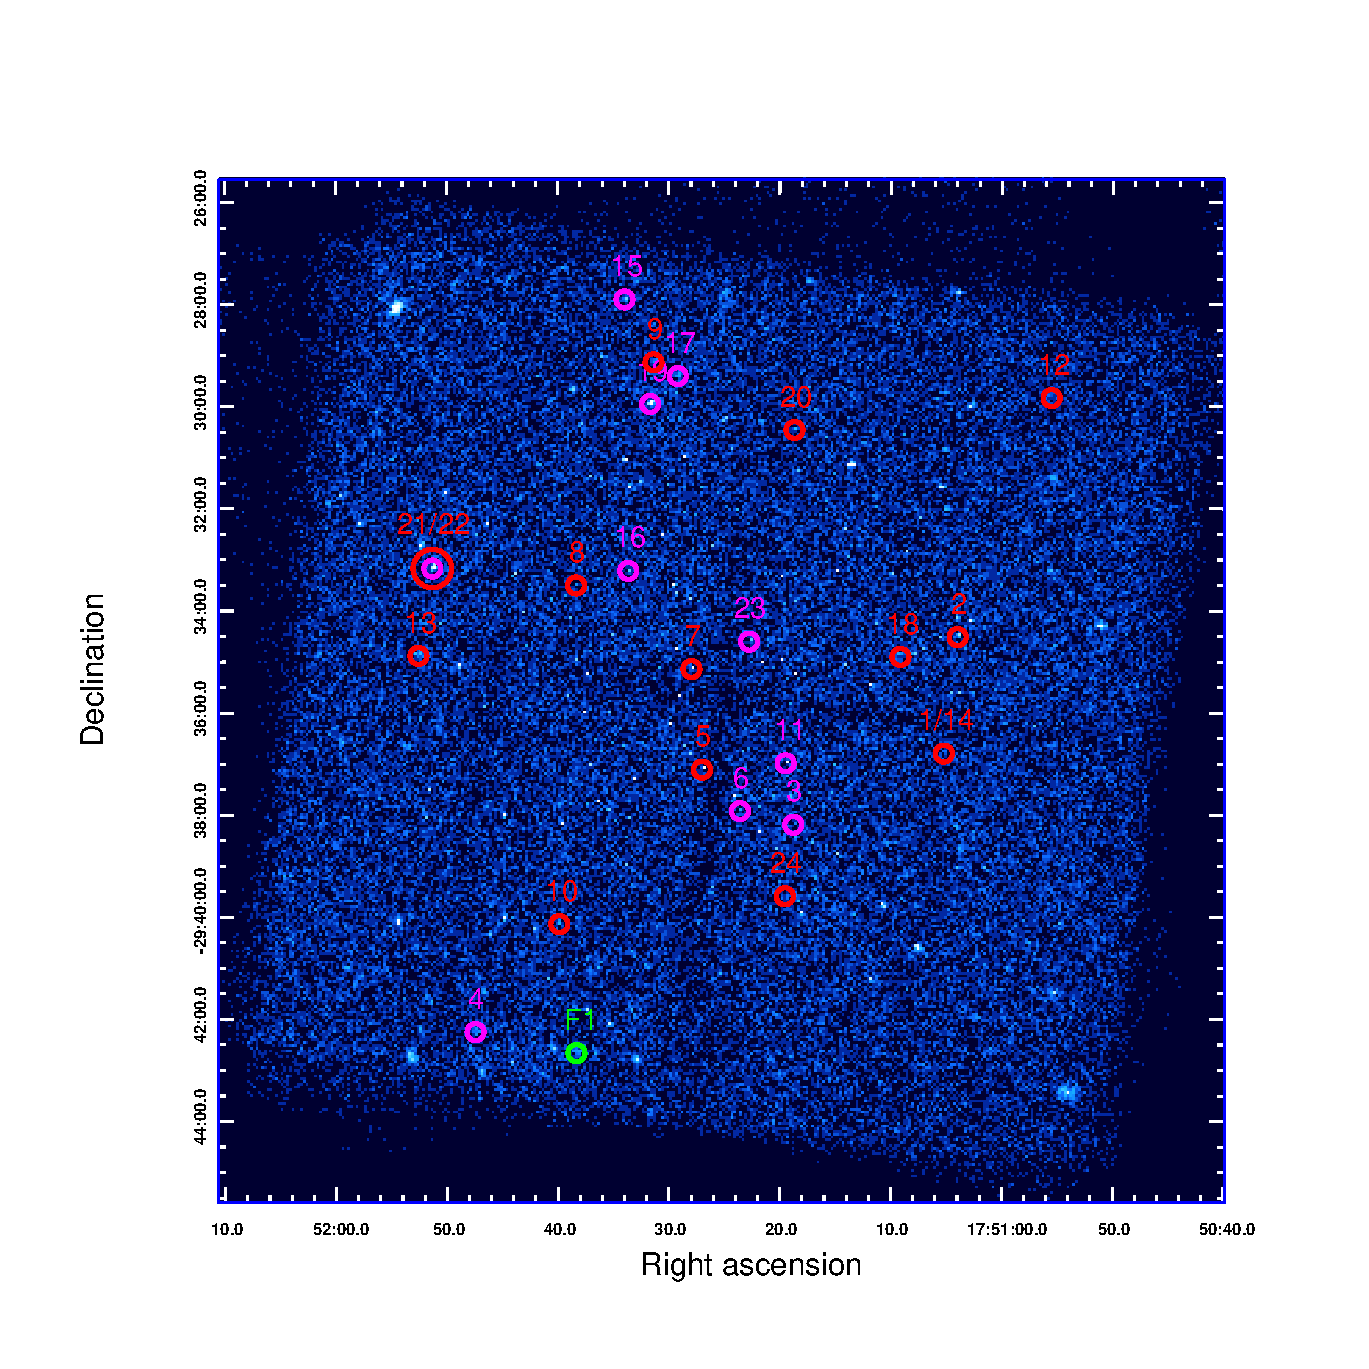
\includegraphics[scale=0.8]{./figure/LW/ds9.eps}
\caption{2--8 keV counts image of the Limiting Window, combining 13 {\it Chandra}/ACIS-I observations. Locations of the 23 periodic sources are marked with colored circles ({\it magenta}: ten sources previously reported by \citealp{2012ApJ...746..165H}; {\it red}: thirteen newly discovered in this work). Source numbering is the same as in Table~\ref{tab:src}. In particular, 1/14 and 21/22 are the two sources each showing two periodic signals.}
\label{fig:FoV}
\end{figure*}

\section{Period Searching Method}\label{sec:methods}
In this section, we first provide our motivation of employing the Gregory-Loredo (GL) algorithm, followed by an outline of its basic principles (Section~\ref{subsec:GL}). We then describe our application of the GL algorithm to the {\it Chandra} data of the LW (Section~\ref{subsec:appli}). This is complemented by a set of simulations to evaluate the detection (in)completeness of periodic signals (Section~\ref{subsec:simulation}).  

\subsection{The Gregory-Loredo Algorithm} \label{subsec:GL}
There exists in the literature a variety of period searching methods, which can be broadly divided into three categories according to their working principles. 

The most traditional method is based on Fourier transform and its power density spectra, which includes the classical Schuster periodogram \citep{1898TeMag...3...13S}, the Fourier analysis with unequally-spaced data \citep{1975Ap&SS..36..137D}, the correlation-based method \citep{1988ApJ...333..646E}, among others.

Another widely-used method seeks to fit the data with a periodic model in the frequency space, employing statistics such as least-squares residuals to define the likelihood function and then selecting the frequency that maximizes the likelihood. The famous Lomb-Scargle periodogram \citep[hereafter LS]{1976Ap&SS..39..447L,1982ApJ...263..835S} belongs to this category. Note that when adopting trigonometric functions, the least-squares method falls into the Fourier transformation category. Another variant is to replace the least-squares residuals with polynomial fits, such as that used in \citet{1996ApJ...460L.107S}.

The last category is the phase-folding method. For each trial period the time-tagged data is folded as a function of phase, and the best-fit period is found by optimizing the cost function through the frequency space. The cost function is designed to evaluate how much the phase-folded light curve deviates from constant.
Methods belonging to this category use diverse cost functions. Several widely known examples are the Epoch Folding (EF) algorithm \citep{1983ApJ...266..160L}, the Phase Dispersion Minimization \citep{1978ApJ...224..953S}, and the GL algorithm \citep{1992ApJ...398..146G}.

In X-ray observations, the detection of periodic signals is often involved with irregularly and sparsely sampled data. 
When working in frequency space, such a sampling can lead to spurious signals and hevay contamination to the real signal. Phase-folding methods, on the other hand, can avoid the effect of non-uniform data since the dead time does not enter the algorithm.
Moreover, the number of detected source counts is often only moderate. While one can in principle apply binning to create photometric light curve, it takes the price of potentially losing temporal information. Phase-folding methods, on the other hand, directly handle individual events, thus maximally incorporating the temporal information.

Most X-ray sources in the LW share the characteristics of irregular sampling and limited source counts. 
Therefore, it is appropriate to employ the GL algorithm, which applies the Bayesian probability theory to the phase-folded light curve, to search for periodic signals for the LW sources. We provide a brief overview of Bayes's theorem and the GL algorithm in Appendix \ref{GL}. 
The key of this algorithm is the multiplicity of the phase distribution of events,
\begin{equation}\label{multi}
W_m(\omega, \phi)={{N!}\over{n_1!\; n_2!\; n_3!\cdots {n_m}!}}.
\end{equation}
Here $N$ represents the total number of counts of a given source, 
%$m$ denotes the number of phase bins, and 
$n_i(\omega, \phi)$ is the number of events falling into the $i$th of $m$ phase bins given the frequency $\omega$ and the phase $\phi$, satisfying $\sum\limits_{i=1}^{m}n_i(\omega, \phi)=N$. 
The multiplicity is the number of ways that the binned distribution could have arisen by chance. It can be easily shown that the more the values of $n_i$ differ from each other, the smaller the multiplicity. In other words, the more the piecewise model defined the $m$ phase bins deviates from constant, the more likely there exists a periodic signal, the probability of which is inversely proportional to the multiplicity.  

In general, the GL algorithm takes the following steps:

(i) Compute the multiplicity for all sets of $(m,\omega, \phi)$ (Eqn.~\ref{multi}). In this work, the highest value of $m$ is set to be 12.

(ii) Given $m$, integrate over the $(\omega, \phi)$ space and calculate the so-called ``odds ratio'' using Bayes's theorem (Eqn.~\ref{A16}). The ``odds ratio'' determines the ratio of probabilities between a periodic model and a non-periodic (constant) model.

(iii) Sum up the normalized odds ratios of each $m$ to determine the probability of a periodic signal (Eqn.~\ref{A20}).
If this probability exceeds a predefined threshold (for instance, 90\%), a periodic signal is favored. 

(iv) Finally, compare all the odds ratios integrated over the $\phi$ space, finding the value of $\omega$ with the highest odds ratio, which then gives the period $P=2{\pi}/\omega$ (Eqn.~\ref{A21}).

%\section{Period searching procedure}\label{sec:timing}
\subsection{Application to the LW}\label{subsec:appli}
We apply the GL algorithm to search for periodic signals in the LW sources. 
For a given source, the 1--8 keV counts within the 90\% ECR of individual ACIS-I observations are extracted to form a time series.  
In addition, we supply for each source the information of ``epoch'', i.e., the start time and end time of each ObsID in which the source has at least one detected count. This information is used to compensate for the uneven distribution over the phase bins (see Eqn.~\ref{A17} for a detailed illustration). 
Since the GL algorithm determines the probability of a periodic signal against a constant light curve, there is no need to separately account for the background level, which is absorbed into the constant. 
Nevertheless, we have measured the local background (Section~\ref{subsec:detect}) for each periodic source as a consistency check (see Section~\ref{sec:results}). 
%Though we did source detection in 2-8 keV band to reduce the contamination from non-CV sources, here we still extracted photons from sources in 1-8 keV band to keep as more as possible source information. 
%Besides, in order to compensate for uneven distribution over the bins, we provide "epoch" for each source. The "epoch" offered the start time and end time of each observations covered the source with at least one counts in source region. See Eqn.~\ref{A17} in appendix for detailed illustration about the use of epoch. 
%For the sake of changing aimpoint, we used individual source extract region for different observations. Explicitly, the 90\% ECR aperture  whose radius defined by specific PSF map was applied for counts in that observation. Since the phase-folding method directly manipulated each photons and we could not distinguish background photon from source photon, the local background information were not provided for timing analysis. The combination of each source event list and the corresponding epoch were then employed as the input of GL method. 

As mentioned in Section~\ref{subsec:GL}, the GL algorithm folds the time series at a trial frequency (or period). 
In practice, the resolution and range of frequency must be compromised between accuracy and computational power. %We choose the frequency range and frequency resolution for the following considerations.
Thus we restrict our analysis on three period ranges: (300, 3000), (3000, 10000) and (10000, 50000) sec, with a frequency resolution of $10^{-7}$, $10^{-8}$ and $10^{-9}$ Hz, respectively. 
The period ranges are chosen based on the expectation that most, if not all, detectable periodic X-ray sources in the LW should be CVs. 
The orbital period distribution of CVs is known to exhibit a minimum at about 82 minutes, a gap between 2--3 hours, and a maximum around 10 hours \citep{2003A&A...404..301R}. 
The second and third period ranges well cover these characteristic periods, whereas the first range probes the spin period of fast rotating IPs.
Given the timespan of $\sim10^8$ sec between the first and last ACIS-I observations, the chosen frequency resolutions are optimal for an efficient search of periodic signals.  

%Ideally, the frequency resolution should keep the phase-folded light curve nearly the same between two adjacent frequencies, that is, the same photon falls within the same phase bin.
%For the data span in timescale T, the arrival time of photon $t_i$ (taking $t_1$=0), the changing angular frequency influence the phase of photon more as $i$ grows. The most "vulnerable" photon is the last photon arrived, whose arrival time is T, and the change of phase is
%\begin{equation}\label{fi}
%\begin{split}
%	d\phi_{N}=&\phi_{N}^{'}-\phi_{N}\\
%	=&[(\omega +d\omega) \cdot T-\lfloor (\omega +d\omega) \cdot T \rfloor] -[\omega \cdot T-\lfloor \omega \cdot T \rfloor]
%\end{split}
%\end{equation}
%\begin{equation}
%	\phi_{N}^{'}=(\omega +d\omega) \cdot T-\lfloor (\omega +d\omega) \cdot T \rfloor
%\end{equation}
%\begin{equation}
%	\phi_{N}=\omega \cdot T-\lfloor \omega \cdot T \rfloor
%\end{equation}
%\end{subequations}
%\\
%Assuming $\lfloor (\omega +d\omega) \cdot T \rfloor = \lfloor \omega \cdot T \rfloor$, ($\lfloor a \rfloor$means the integral part of a), then 
%\begin{equation}
%	d\phi_{N}=d\omega \cdot T
%\end{equation}
%In this work, we take 12 as the largest number of phase bins, that demands the change of photon phase should be smaller than the length of bin, i.e, ${1\over 12}\cdot 2\pi $, to guarantee the nearly non-change of phase-folded light curve. Although we can not ensure every photon to meet the requirement since its location in the same phase bin could be arbitrary. It would satisfy the situation at nearly perfect level if we keep the deviation of phase of last photon smaller than ${1\over 12}\cdot 2\pi $. As shown in Eqn.~\ref{dfi}
%\begin{subequations}\label{dfi}
%\begin{equation}
%	d\phi_{N}=d\omega \cdot T< {1\over 12}\cdot 2\pi
%\end{equation}
%\begin{equation}
%	d\omega < {{\pi}\over {6\;T}}
%\end{equation}
%\end{subequations}

%The total span of 13 observation is about three years, i.e., $10^8$ s, so the resolution of angular frequency is $5\times 10^{-9}$. When the $\omega$ increases, corresponding the period decreases, the same resolution brings numerous discrete frequencies and raises running time greatly. 
%Thus we used three different resolutions $10^{-7},10^{-8},10^{-9}$ in three period ranges $(300s,3000s),(3000s,10000s), (10000s,50000s)$. The ranges was chosen for the orbital period distribution of CVs, as shown in Figure \ref{fig:N_P}. There is a period gap in distribution at 2-3 hours, and a period minimum at about 70 minutes. Then the first range covers roughly the spin period of IPs, the other two ranges overlay the orbital period below and beyond the period gap respectively.

%Generally, for each source, we provide the dataset for GL method. Then we got the most periodic signal with its probability in three period ranges. Taking 90\% as threshold to determine the periodicity, finally we choose all the candidate sources with at least one periodic signal.

\subsection{Detection completeness}\label{subsec:simulation}
For a given period searching algorithm, the detection rate depends on both the number of observed counts, the intrinsic shape of the light curve, as well as the observing cadence. 
To quantify the detection rate and hence gain insight on the nature of the periodic sources in the LW, we perform simulations following the merit of \citet{1998ApJ...498..666C}. 
Two functional forms of light curve are considered: a sinusoidal function and a piecewise function. While these are admittedly idealized shapes, they can represent realistic light curves, e.g., the former resulted from rotational modulation and the latter due to eclipse. 

A sinusoidal light curve follows,
\begin{equation}
\lambda (t)=\lambda_0[1+A_{0}{\rm sin}(\omega t+\phi)], 
\label{eqn:sin}
\end{equation}
where $\omega = 2{\pi}/P$, $A_0$ is the relative amplitude of variation, and $\lambda_0$ is the mean count rate which may include contribution from a constant background. The phase $\phi$ can be arbitrarily set at zero.
For a direct comparison with observations, we relate $\lambda_0$ with the total number of counts, $C = \lambda_0 T$, where $T$ is the exposure time of a given observation. This holds since $T$ is typically much longer than the modulation period ($P$). 
The simulations are run with a selected number of parameters due to constraints in computational power. 
Specifically, we adopt $C$=50, 100, 200, 300, 400 and 500, $A_0$=0.5, 0.6, 0.7, 0.8 and 0.9, and $P$=554, 5540 and 45540 sec, resulting in a total of 6x5x3=90 combinations. 
The chosen periods are representative of the actually searched ranges (Section~\ref{subsec:appli}), whereas
the adopted total counts well sample the range of observed counts from the LW sources.

We thus simulate 100 light curves for each combination of parameters, taking into account Poisson errors and the exact start and end times of the 13 ACIS-I observations. The arrival time of each simulated count is further randomly modified by an amount of 3.2 sec to mimic the effect of ACIS frame time.
The simulated light curve is then searched for a periodic signal using the GL algorithm in the same manner as for the real data (Section~\ref{subsec:appli}).
We count a valid detection if the found period has a detection probability greater than 90\% and its value consistent with the input period to within 1\%. 
%Besides, the harmonics have also been considered as valid detection  with the same threshold, i.e, the deviation between determined period and resonance cycle within 1\%.
We notice that in a small fraction of simulated light curves of the shortest input period (554 sec), the second harmonics (i.e., 2 times the true period) is detected with an even higher probability than the true period. We also consider such cases a valid detection as long as the true period itself fulfills the above criteria.
%In our simulation, the effect of harmonics only happens in the first period range due to the selection of parameter value, with fraction of harmonics detection about 20\%, concentrated at higher amplitude.
%For completeness, we ran the same process at $P$=4000 sec and $P$=20000 sec, adopting $C$=500 and $A_0$=0.9, and found there is no harmonics detection.

The detection rate for a given combination of parameters is taken to be the fraction of the 100 simulated light curves having a valid detection. The top, middle and bottom panels of Figure \ref{fig:detection} show the result of the three test periods, respectively, in which several trends are apparent. 
First and intuitively, for a given period and amplitude, higher total counts would lead to higher detection rates, while for given total counts, a higher amplitude also leads to a higher detection rate. The simulation results confirm these expectations.  
Second, for the same total counts and amplitude, the detection rate is generally higher for a longer period.  
This can be understood as due to a statistical behavior in the 
multiplicity (see Eqn.~\ref{multi}), which has a lower value for a long period. This holds for both the sinusoidal and piecewise light curves. 
%it can be seen that the algorithm is nearly no bias of period, except a slight improvement of detection rate with increasing period. We exhaust every possibility to figure out the origin of improvement. After trial simulation, it turns out that statistically the multiplicity (Eqn.~\ref{multi}) has lower value with longer period, contributing to higher detection rate. Mathematically, this is due to the integral over time of counts rate (see Eqn.~\ref{eqn:sin}). The integral process brings about the value of deviation, between constant and variation, proportional to signal period because of the contribution of $w$ on denominator, resulting the negative association between multiplicity and period.
Lastly, for total counts of 50, the detection rate is almost always below 10\% regardless of the period and amplitude. 
%The periodic signal in this circumstance could be unreliable.
%With more counts, the detection rate can exceed 50\%, which is sufficient enough for period finding procedure. 
 
\begin{figure}
\begin{minipage}[b]{0.45\textwidth}
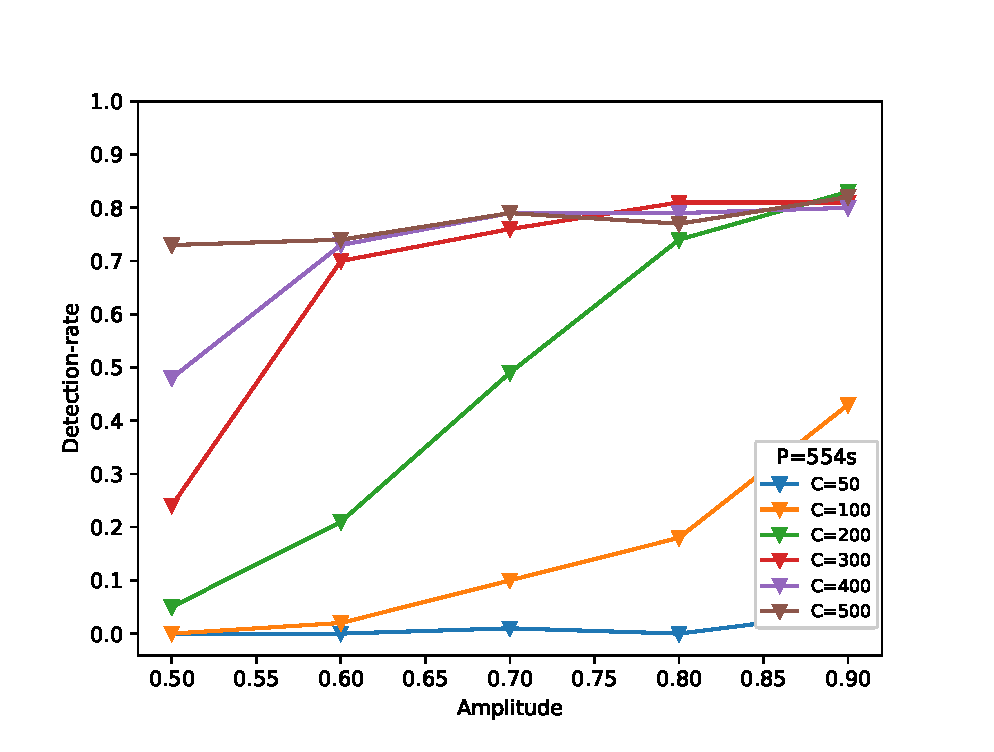
\includegraphics[width=\textwidth]{./figure/sim_LW/detection_554.eps}
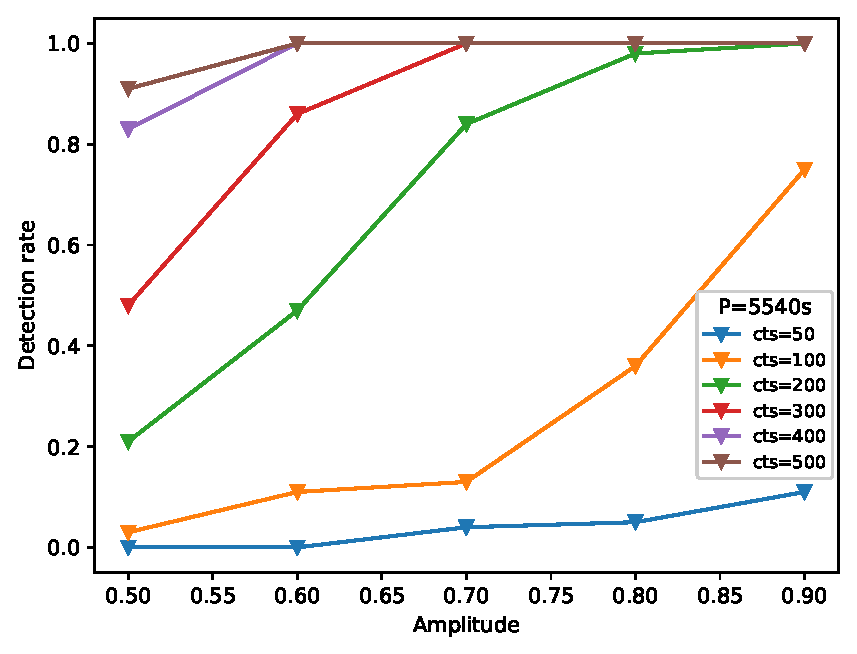
\includegraphics[width=\textwidth]{./figure/sim_LW/detection_5540.eps}
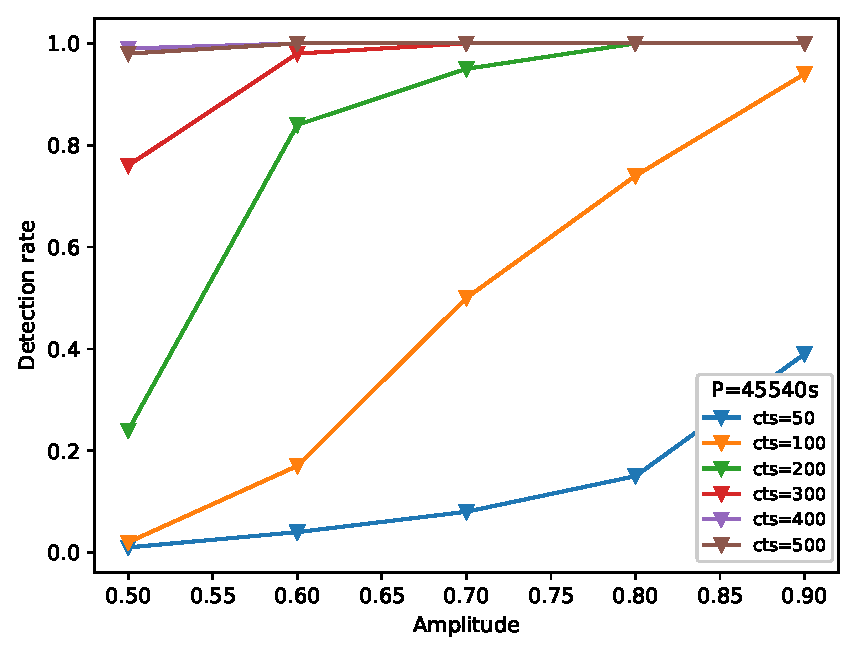
\includegraphics[width=\textwidth]{./figure/sim_LW/detection_45540.eps}
\end{minipage}
\caption{Detection rates as a function of relative variation amplitude, based on simulated sinusoidal light curves. The top, middle and bottom panels are for modulation period of 554, 5540 and 45540 sec, respectively. The different colored lines represent different values of total counts, as labeled. See text for details.
\label{fig:detection}}
\end{figure}

The piecewise function, which mimics an eclipse against an otherwise constant flux, takes the form of
\begin{equation}
\lambda(t)=
\begin{cases}
\lambda_0 & \text{$\phi(t) \in[0,(1-w)\pi)\cup ((1+w)\pi,2\pi]$},\\
f\lambda_0 & \text{$\phi(t) \in[(1-w)\pi,(1+w)\pi]$},
\end{cases}	
\end{equation}
where $w$ accounts for the eclipsing width (duration) in phase space, and $f$ characterizes the relative depth of the eclipse ($0\leq f \leq 1$; $f = 0$ corresponds to total eclipse). Here the middle of eclipse is assumed to occur at $\phi = \pi$. 
Again, $\lambda_0$ can be related to the total counts as $C=[1-(1-f)w]\lambda_0T$.
We set $f=0.1$ and $w=0.1$ in our simulations, which are not atypical of eclipsing CVs. 
%since the radius ratio of WD, companion star and orbit are about 1:10:50. 
We test three values of the period, $P$=5258, 15258 and 45258 sec and adopt trial count rates $\lambda_0 = 1, 2, 3, 4, 5, 6, 7, 8, 9, 10, 15$ and $20\times10^{-4}{\rm~cts~s^{-1}}$.
For each combination of parameters, 100 simulated light curves are again generated and fed to the GL algorithm. 
The resultant detection rate (also taking 90\% as the threshold) is shown in Figure~\ref{fig:eclipse}. 
As expected, the detection rate is generally higher for a longer period.
It can also be seen that for total counts below $\sim$300, the detection rate is $\lesssim$10\% regardless of the period; only when total counts exceed $\sim$1500, the detection rate becomes 100\% for all test periods. 
Since only a small fraction of sources in the raw list have total counts more than 1500, we expect a relatively low detection rate of eclipsing sources in the LW.  
 
\begin{figure}
\centering
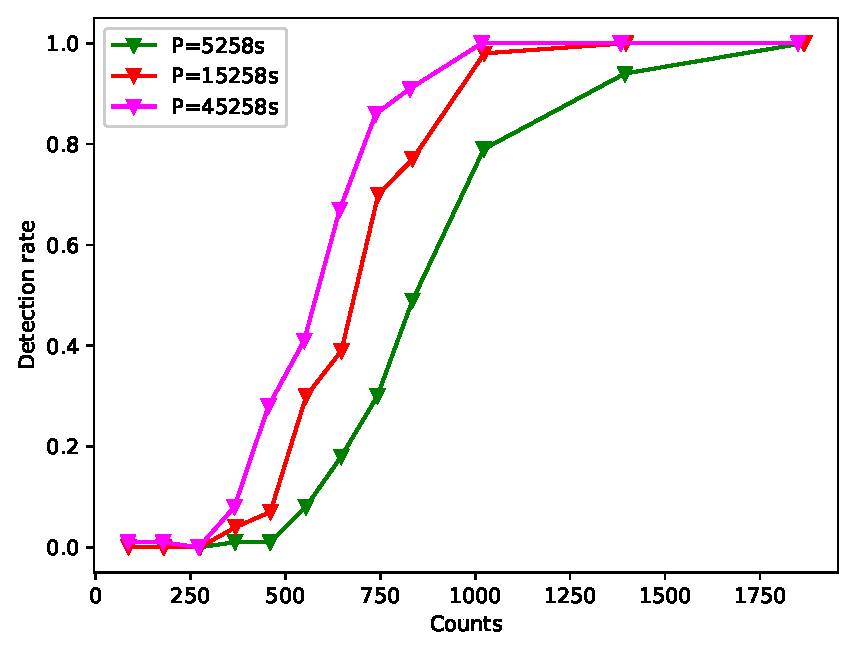
\includegraphics[scale=0.61]{./figure/sim_LW/eclipse_cut.eps}
\caption{Detection rates as a function of total counts, based on simulated piecewise light curves. Different colored lines represent different periods, as labeled. See text for details.}\label{fig:eclipse}
\end{figure}

We have also run simulations to estimate the rate of false detection, which refers to the detection of a periodic signal from an intrinsically constant light curve. 
Considering that most LW sources can have a low-amplitude long-term variation, we approximate a semi-constant light curve with a sinusoidal function with $P$=5 yr and $A_0$=0.5. 
Simulated light curves are generated with totals counts from 50 to 5000 and fed to the GL algorithm. No false detection of periodic signals, at any value between 300--50000 sec, is found. 
Therefore, it seems safe to conclude that the false detection rate is essentially zero for the GL algorithm applied to the LW data. 

\section{Period Searching Results}\label{sec:results}
%\subsection{Filtering detections}
According to the simulations in Section~\ref{subsec:simulation}, a periodic signal is hard to detect in LW sources with total counts $C<100$, even in the case of high variation amplitudes.  
Therefore, we restrict our period searching to sources with $C \geq 100$, which include 667 of the 847 sources in the raw list.Among these 667 sources, 25\% (4\%) have total counts more than 500 (1000).

Adopting a probability threshold of 90\%, we obtain 48 tentative periodic signals from the three period ranges. However, it is necessary to filter spurious detections, which may be caused by several effects:

(i) By design, the ACIS is dithered to distribute photons over more CCD pixels to avoid pile-up and to fill CCD gaps. The dither period is 706.96 s in pitch and 999.96 s in yaw. Any signal detected at these two periods and their harmonics are thus excluded. These are mostly found in sources located close to CCD gaps, where dithering significantly reduces the number of detected counts in a periodic fashion. 

A related concern is how dithering would affect the detection of genuine periods.  
We run simulations to test this effect. Specifically, we generate simulated sinusoidal light curves with $P$ = 5072.97 sec and $C$ = 293. 
This choice is motivated by one particular periodic source (\#5 in Table~\ref{tab:src}), which has a fractional detector coverage of 0.74 (in other words, 26\% of the intrinsic flux is lost due to dithering into the CCD gap), the lowest among all valid periodic sources (see below). The dithering effect is mimicked by artificially removing the simulated counts according to a probability distribution calculated by the CIAO tool \emph{dither\_region}. 
No difference is found in the resultant detection rate, compared to that without dithering. 
%Out of concern about the dither effect on period searching, we compute the fractional area covered by chips (hereafter FA) for each source in each observation. FA equals 1 when source region are not affected by gaps. After, weighting the FA in total exposure time, we define $\overline{FA}$ for each source. Most of $\overline{FA}$ are beyond 0.9, except for \#5, which is 0.74. Thus we run 100 simulation for this source in two cases. One for no dithering and the other for dithering. It turns out no difference in detection rate. In general, we can neglect the dither effect. 

(ii) In certain sources, multiple detections can be caused by second and third harmonics of the same intrinsic signal (i.e., 2 and 3 times the true period). These can be easily identified by the sign of double-peak or triple-peak in the phase-folded light curve, provided that the intrinsic signal has a single-peak structure. 

However, the intrinsic structure might be double-peaked, in which case it is more difficult to distinguish between the true period and the half harmonic (i.e., half the true period), in particular when the two peaks have a similar strength and width.
Generally speaking, the double-peaked shape only occurs in IPs with an accretion column over each magnetic pole. When viewed from certain angle, the two poles alternatively drift across the front side of the WD, producing the double-peaked X-ray light curve. The modulation period in this case must be the spin period of the WD, typically under one hour. Among our tentative detections, most of those showing a double-peaked light curve have a corresponding period longer than 3 hours, far beyond the range of spin periods in IPs. 
These are probably second harmonics rather than a genuine spin period. 
Hence we assume that there is no half harmonics in the LW sources and always take the lowest period as the true period. This assumption is supported by our extensive simulations presented in Section~\ref{subsec:simulation}, in which no half harmonic (the true period is known before hand) is found.  
%Appendix~\ref{harmonics} provides more discussions about harmonics.

(iii) Strong flux variations or outbursts occupying one particular observation can also cause a false periodic signature. This is because the GL algorithm, which analyzes the phase-folded light curve, can be fooled if there were too many photons found in a single observation, producing excess in certain phase bins. In this case the algorithm may ``think'' there exists a period especially in the period range of (10000, 50000) sec. Among the sources with tentative periods, four exhibit a variability index VI$>10$, indicating strong variations. We thus reanalyze their light curves using two subsets of observations: those covering only the outburst and those excluding the outburst. For three of them, the tentative period cannot be recovered in either subset. Therefore, these three are probably fake signals. The remaining source is retained since its period can be recovered in both the outbursting and quiescent subsets.

%\subsection{Confirmed Periods}
The above filtering thus results in 25 valid periodic signals in 23 sources.
Among them, 10 signals were previously reported by \citet{2012ApJ...746..165H} and are confirmed here with the GL algorithm, while the remaining 15 periods are new discoveries (a comparison between our work and \citealp{2012ApJ...746..165H} is further addressed in Section~\ref{subsec:compare}). 
The basic information of these periodic sources are listed in Table~\ref{tab:src}, sorted by the order of increasing period. The source locations are marked in Figure~\ref{fig:FoV}.

Two sources each exhibit two different periods, hence we have assigned each of them two IDs: \#1/\#14 and \#21/\#22.  
The phase-folded light curves at the two modulation periods are shown for source \#1/\#14 in the upper panels of  Figure~\ref{fig:pCV_sample_1} and for source \#21/\#22 in the upper panels of Figure~\ref{fig:pCV_sample_2}. 
The number of phase bins, between 20 to 50, is chosen to optimally display substructures in the light curve. While the GL algorithm does not rely on quantifying the local background, for comparison we plot in these panels the estimated background level (yellow strip, the width of which represents 1\,$\sigma$ Poisson error; Section~\ref{subsec:detect}). 
We defer discussions on the shape of the light curve, which contains important information on the nature of the periodic sources, to Section~\ref{subsec:class}. 
 
The phase-folded light curves are complemented by the long-term, inter-observation light curve, shown in the lower left panel of Figures~\ref{fig:pCV_sample_1} and \ref{fig:pCV_sample_2}, 
and by the source spectrum (see Section~\ref{sec:spectra}),
shown in the lower right panel of Figures~\ref{fig:pCV_sample_1} and \ref{fig:pCV_sample_2}. 
%For middle panel, the valid detection (defined in \ref{subsec:detect}) are plotted with dots plus error range. While the non-valid detection are shown in arrows, providing only the upper limits. Meanwhile, the x-axis in right panel were plotted in discontinuous style for better demonstration effect, since the short interval over the last eight observations. 
%For right panel, the spectra illustrated here were fitted in the range of 1--8 keV, consistent with the timing analysis. 
Similar figures of the remaining 21 sources are presented in Appendix~\ref{appen:fig}.

\begin{table*}
\centering
\begin{threeparttable}
\caption{Information on the periodic X-ray sources in the Limiting Window \label{tab:src}}
\begin{tabular}{lcccccccccccc}
\hline
\hline
ID& R.A. & Decl. & Period & Prob. & $C$ & VI & H-ID  & $P_{\rm det}$ & Harmonics & Class 
\\
LW & $\circ$ & $\circ$ & s & &  &  & \% & &
\\ 
(1) & (2) & (3) & (4) & (5) & (6) & (7) & (8) & (9) & (10)  & (11)
\\
\hline
1$^\dag$ & 267.77173 &	-29.61332 & 853.83 & 0.90277 & 202 & 1.92 &- &- &- 
& IP
\\
2 & 267.76657 &	-29.57529 & 3820.83 & 0.99222 & 902  & 1.94 &- & - &- & IP?
\\
3 & 267.82829 &	-29.63660 & 4728.90 & 1.00000  & 394 & 2.13  & H6 & 99  & \text{Third} & IP?
\\
4 & 267.94766 &	-29.70427 & 4886.79 & 0.99994  & 784  & 1.90 &H8 & 98  &- 
& polar?
\\
5 & 267.86255 &	-29.61859 & 5072.97 & 0.99933 & 293 &  2.34 &-& - &\text{Second} & polar?
\\
6 & 267.84831 &	-29.63212 & 5130.57 & 1.00000  & 437 & 2.51  & H2 & 100 & \text{Second} & polar?
\\
7 & 267.86651 &	-29.58575 & 5144.97 & 0.99880 & 335 & 2.48 &-&-
& \text{Second} & IP?
\\
8 & 267.90982 &	-29.55845 & 5158.75 & 1.00000 & 121  & 2.30 &-&- & \text{Second} & polar?
\\
9 & 267.88075 &	-29.48562 & 5231.49 & 0.94949 & 347  & 1.65 &-&- &- & polar?
\\
10 & 267.91616 &	 -29.66900 & 5252.93 & 0.91425 & 211 
	 &-&-&-&-& polar?
\\
11 & 267.83116 &	 -29.61651 & 5261.93 & 1.00000 & 438 & 1.46 & H10 & 31 & \text{Second} & IP?
\\
12 & 267.73141 &	 -29.49721 & 5334.76 & 0.99952 & 760 & 1.25 
	 &- &- & \text{Second} & polar?
\\
13 & 267.96901 &	 -29.58142 & 5501.16 & 0.99094 & 512 & 2.89
	 &- &- &- & polar?
\\
14$^\dag$ & 267.77173 & -29.61332 & 5608.21 & 0.96821 & 202  & 1.92 
 &-&-& \text{Third} & IP
\\
15 & 267.89161 &	 -29.46508 & 6335.85 & 1.00000 & 823 & 2.09  & H5 & 100  & \text{Second} & polar?
\\
16 & 267.89024 &	 -29.55369 & 6597.55 & 1.00000 & 487  & 4.30  & H9 & 99 & \text{Second} & polar?
\\ 
17 & 267.87162 &	 -29.49011 & 7448.98 & 0.99999  & 535 & 1.76  & H3 & 100 & \text{Second} & polar?
\\
18 & 267.78806 &	 -29.58177 & 7756.19 & 0.99941 & 214  & 4.76 &-&- &\text{Second} & IP?
\\
19 & 267.88203 &	 -29.49922 & 8546.28 & 1.00000  & 3402  & 3.27 &H4 & 93  & \text{Second} & IP?
\\
20 & 267.82785 &	 -29.50770 & 8844.82 & 0.90987 & 263 & 1.82
	&- &- & \text{Second} & IP?
\\
21$^\ddag$ & 267.96375 & -29.55290 & 9877.52 & 0.99992  & 1963 & 1.44 & - &- &- & IP
\\
22$^\ddag$ & 267.96375 & -29.55290 & 10342.30 & 1.00000 & 1963  & 1.44 & H1 & 99 &- & IP 
\\
23 & 267.84487 &	 -29.57680 & 12002.70 & 1.00000 & 307 & 1.86 & H7 & 100 & \text{Second} & polar?
\\
24 & 267.90974 &	-29.71112 & 42219.03 & 1.00000  &1039 &23.6 & - &- &- & polar?
\\
25 & 267.83142 &	 -29.65992 & 47317.12 & 0.98850 & 138  &- &- &- &- & AB
\\
\hline
\end{tabular}
\begin{tablenotes}
      \small
      \item 
      Notes:
      (1) Source sequence number assigned in the order of increasing period. The same source with dual periods is marked by \dag\ and \ddag. 
(2) and (3) Right Ascension and Declination (J2000) of the source centroid. 
(4) The modulation period determined by the GL algorithm.
(5) The probability of the periodic signal defined by Eqn.~\ref{A20}.  
(6) The number of total counts in the 1-8 keV band.
(7) The long-term variability index, defined as $\rm VI=S_{max}/S_{min}$, where $\rm S_{max}$ and $\rm S_{min}$ are the maximum and minimum photon fluxes among all the valid detections. Sources \#10 and \#25 have no measurable VI.
(8) The ID of previously detected periodic signals as given table 2 of \cite{2012ApJ...746..165H}.
(9) The detection probability with the GL algorithm based on simulated sinusoidal light curves.
(10) Significant harmonics, when present.
(11) Source classification based on the phase-folded light curve.
\end{tablenotes}
\end{threeparttable}
\end{table*}

\begin{figure*}
\begin{minipage}[t]{0.45\textwidth}
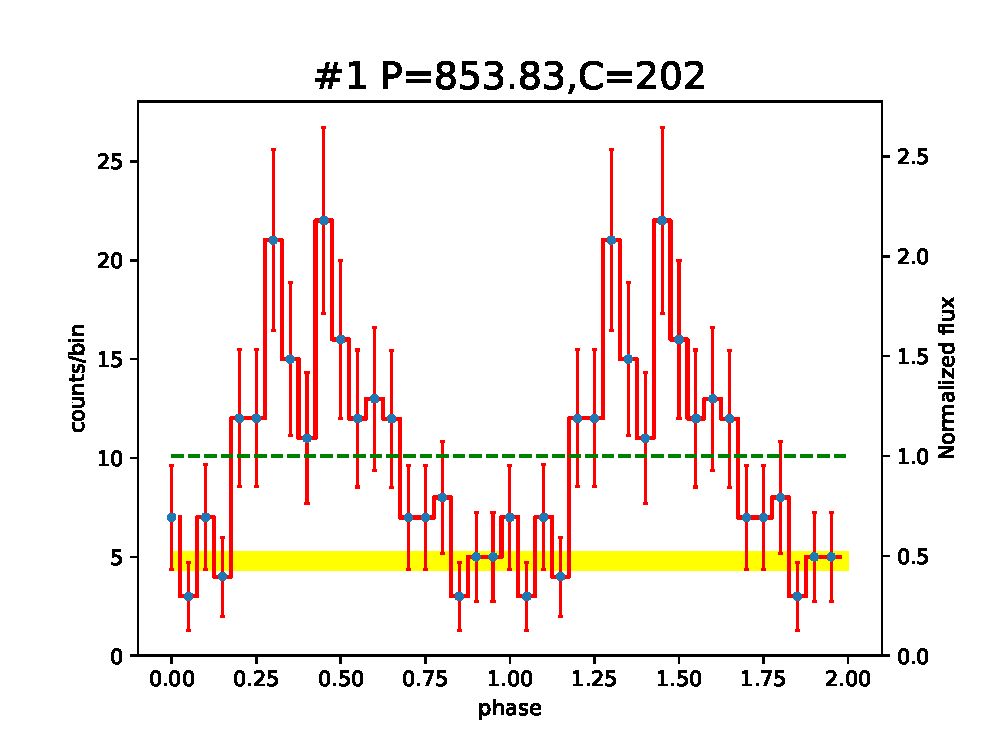
\includegraphics[width=\textwidth]{./figure/LW/pfold_lc_324001.eps}
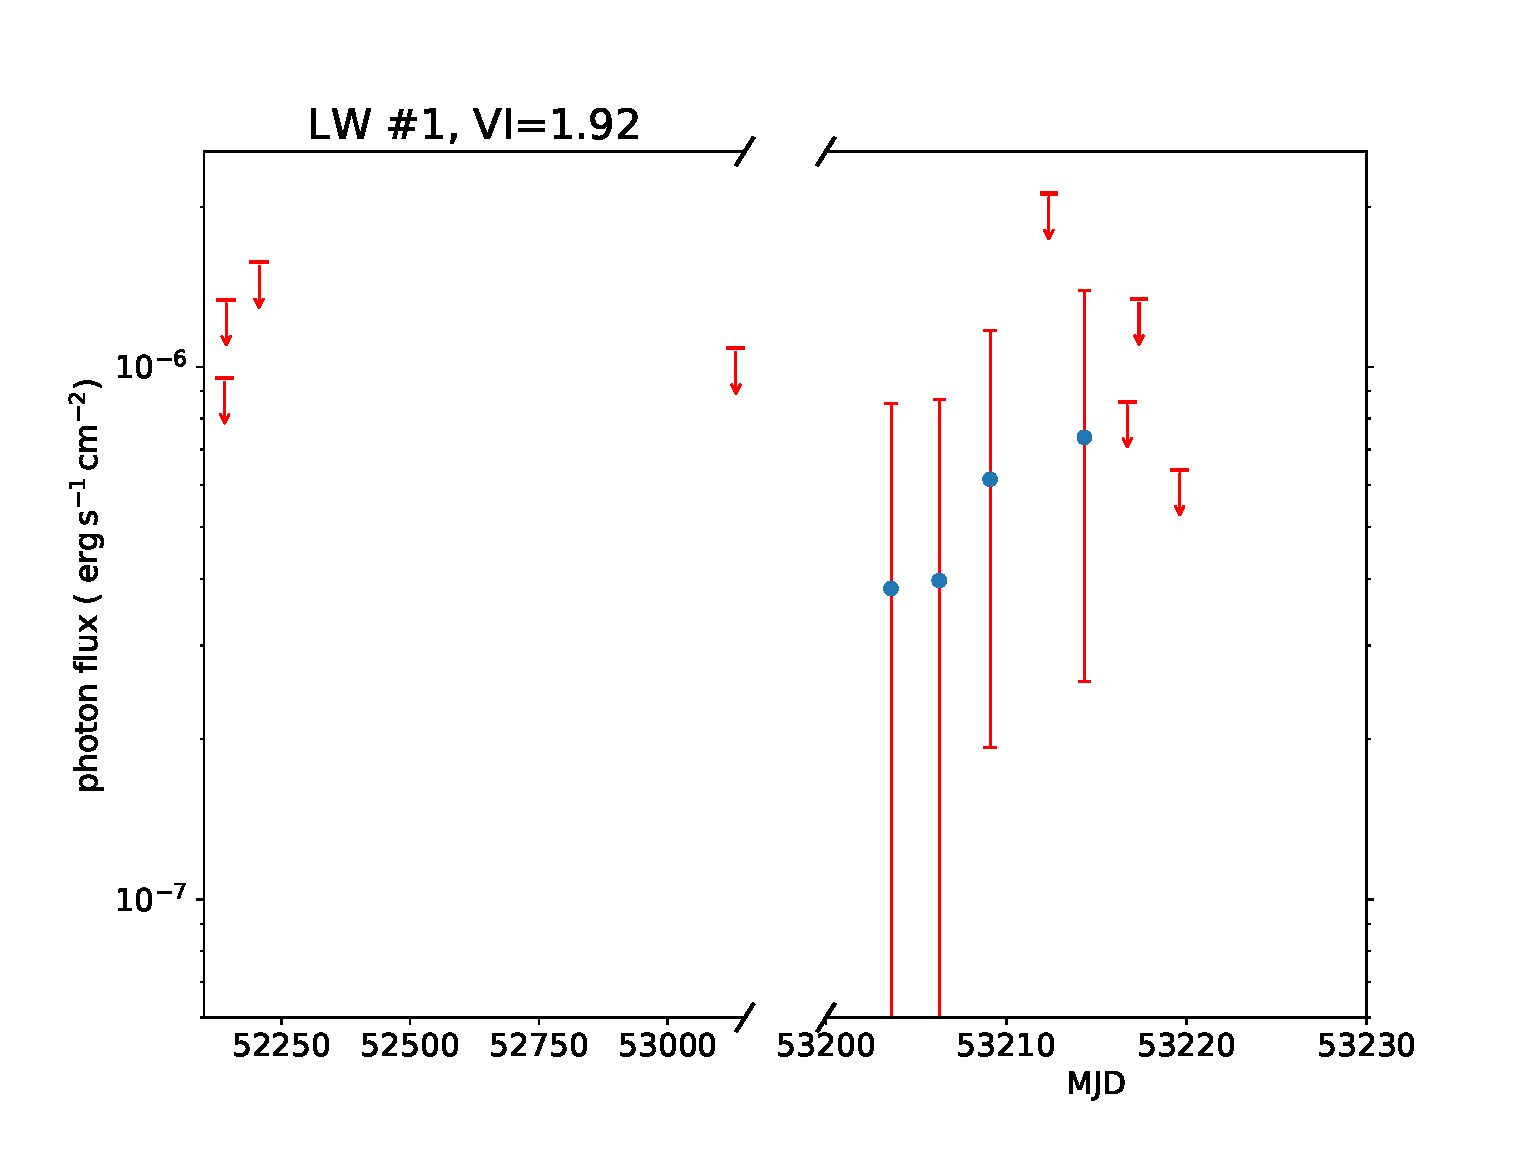
\includegraphics[width=\textwidth]{./figure/LW/324001_lc.eps}
\end{minipage}
\begin{minipage}[t]{0.45\textwidth}
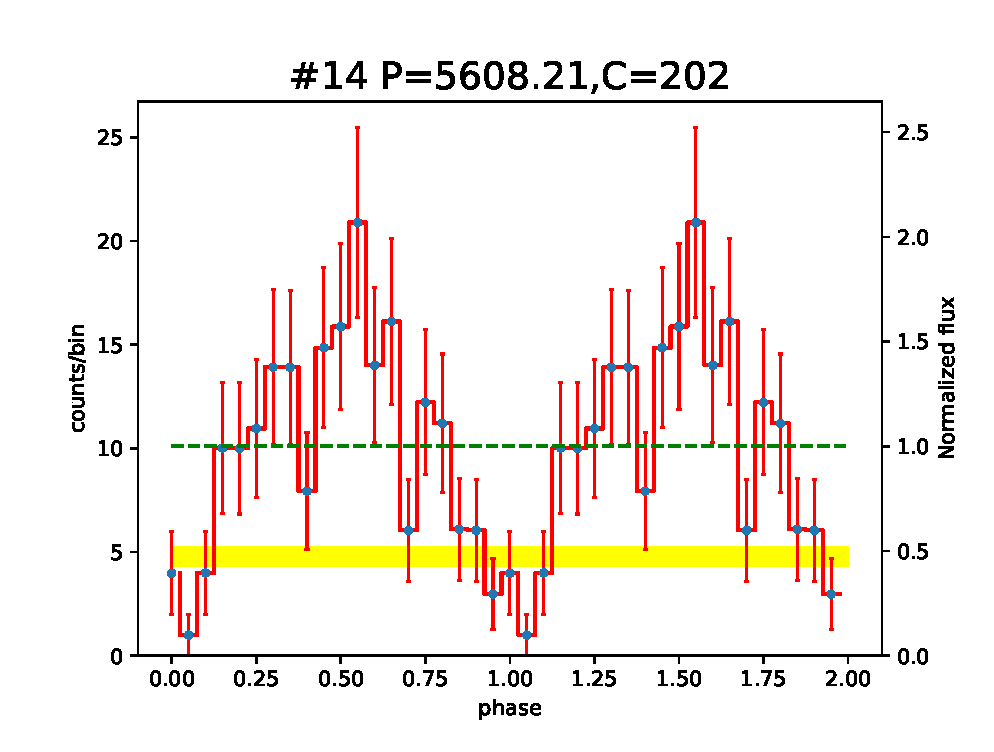
\includegraphics[width=\textwidth]{./figure/LW/pfold_lc_324002.eps}
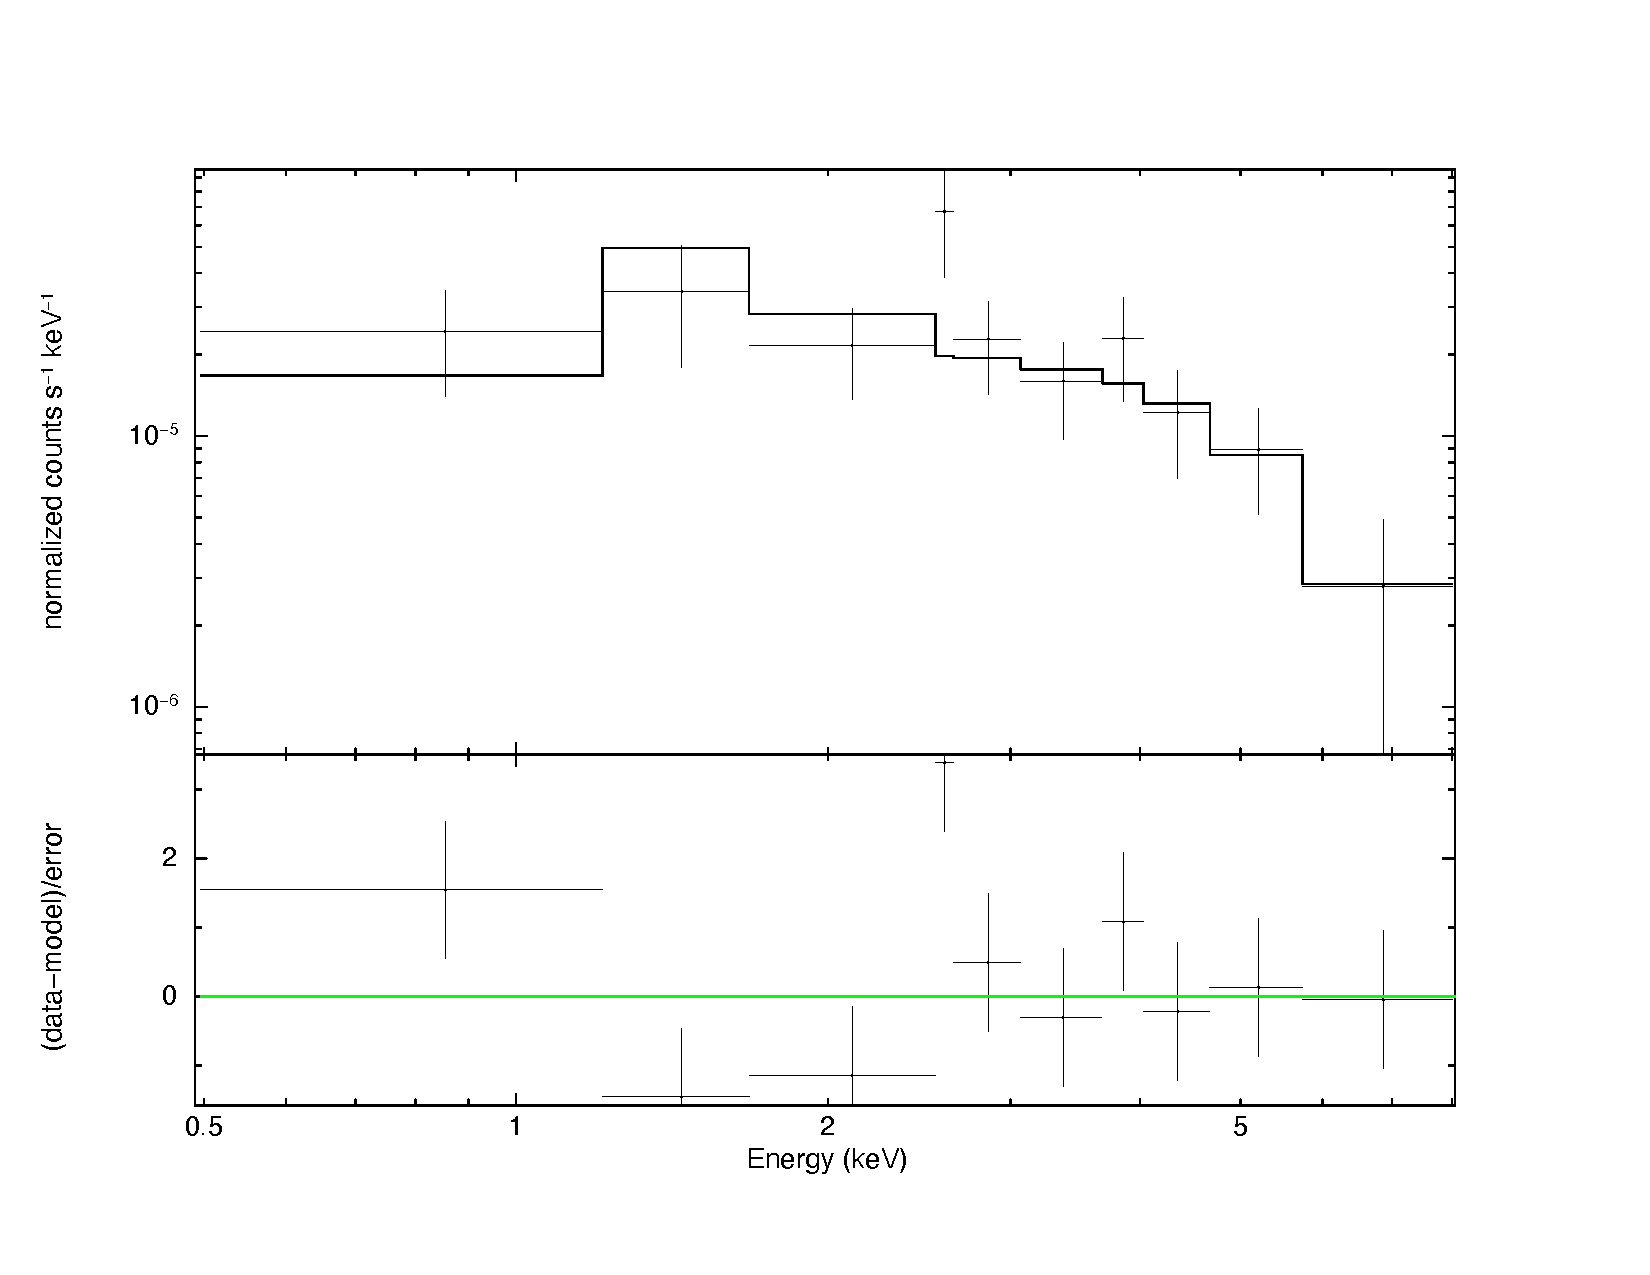
\includegraphics[width=1.02\textwidth]{./figure/LW/324001_spec.pdf}
\end{minipage}
\caption{{\it Upper panels}: The 1--8 keV phase-folded light curves of source \#1/\#14 at the two modulation periods.
The green dashed line represents the mean count rate, whereas the yellow strip represents the local background, the width of which represents 1\,$\sigma$ Poisson error.
{\it Lower left}: the 1--8 keV long-term, inter-observation light curve. Arrows represent 3\,$\sigma$ upper limits. 
{\it Lower right}: Source spectrum and the best-fit model. See text for details.}
\label{fig:pCV_sample_1}
\end{figure*}

\begin{figure*}
\begin{minipage}[t]{0.45\textwidth}
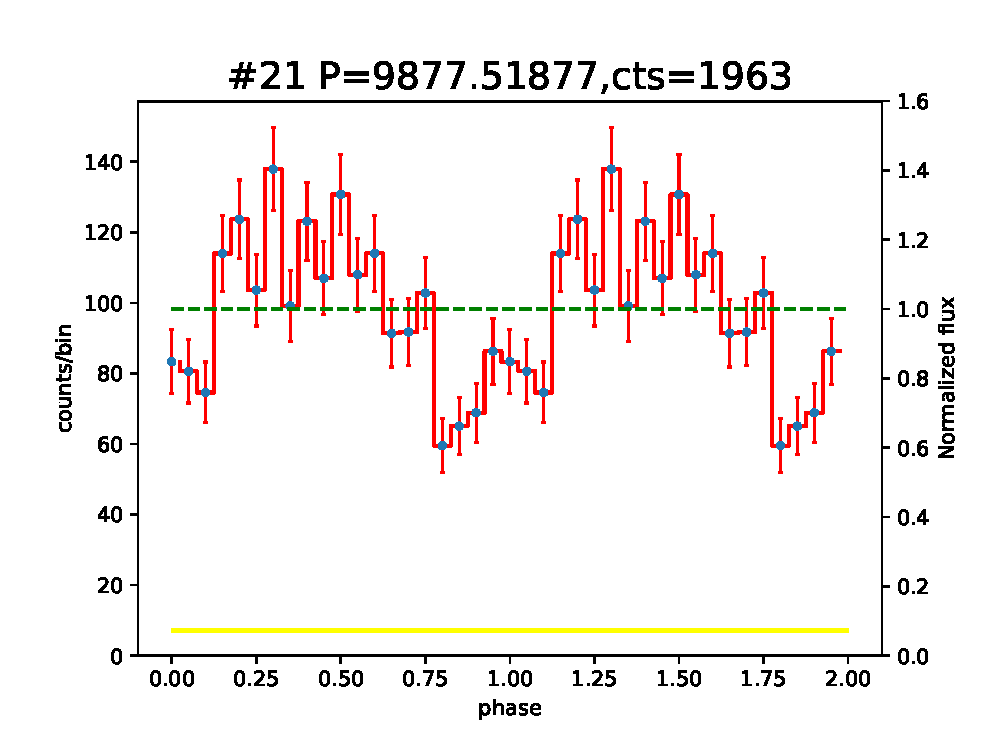
\includegraphics[width=\textwidth]{./figure/LW/pfold_lc_153001.eps}
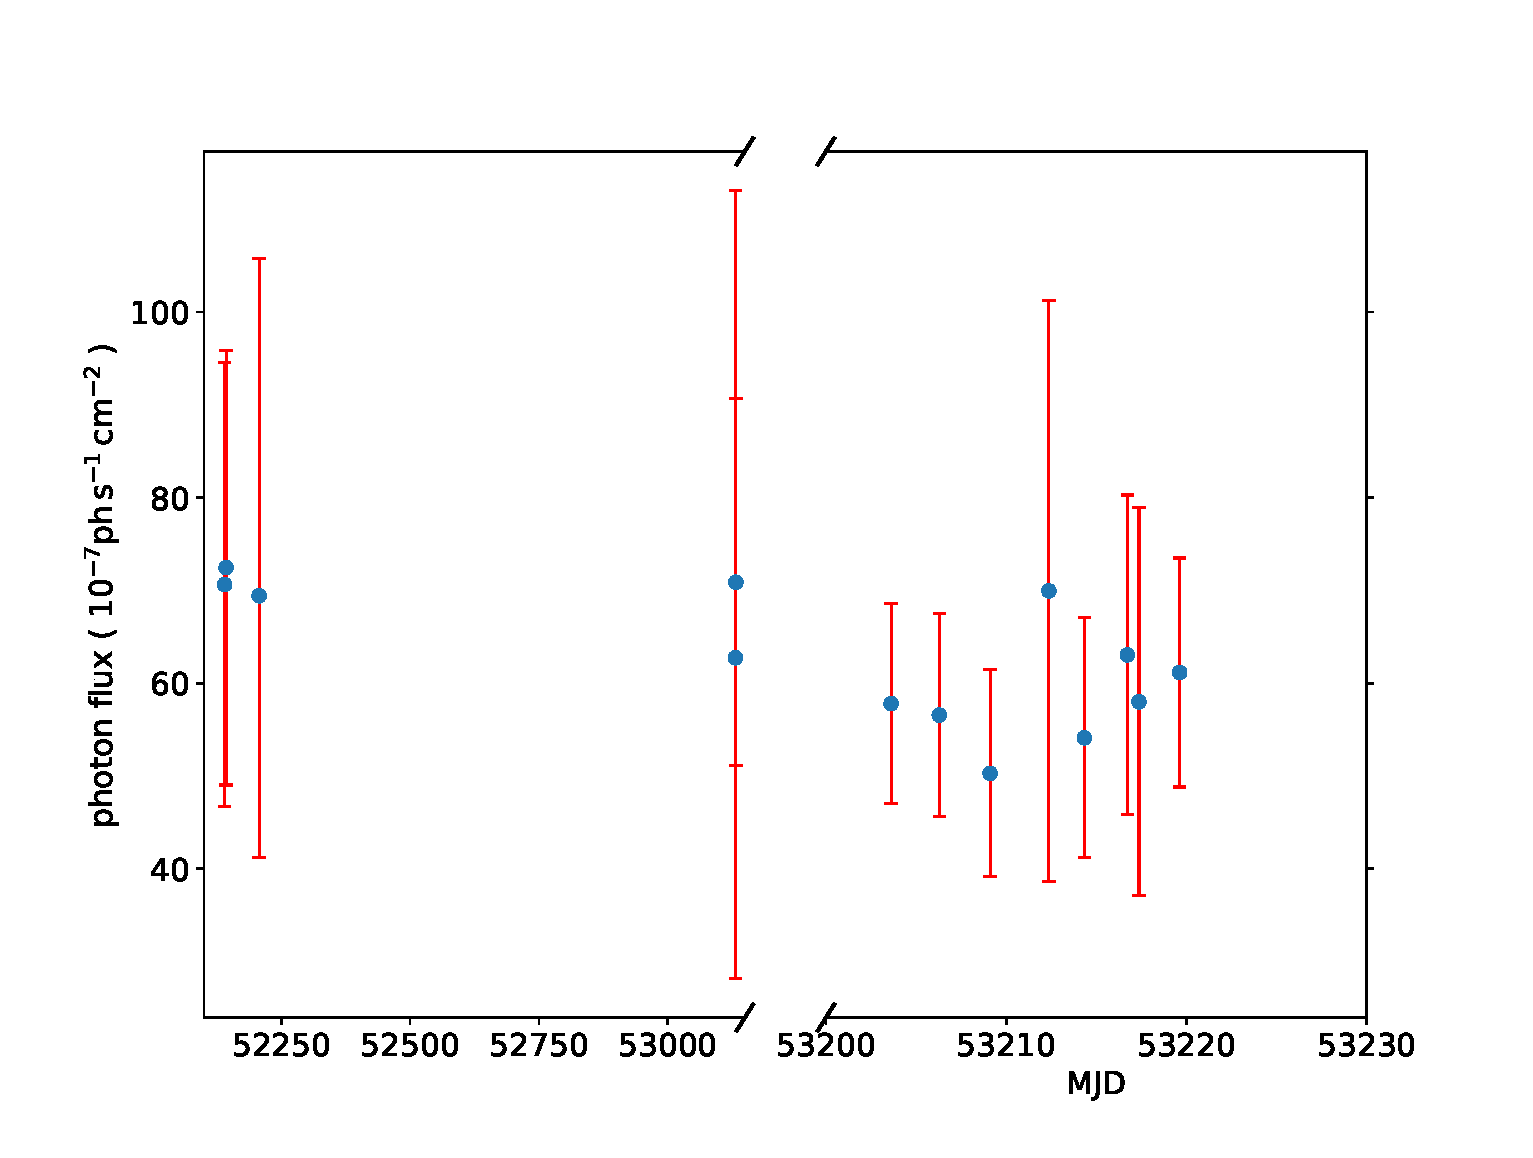
\includegraphics[width=\textwidth]{./figure/LW/153001_lc.eps}
\end{minipage}
\begin{minipage}[t]{0.45\textwidth}
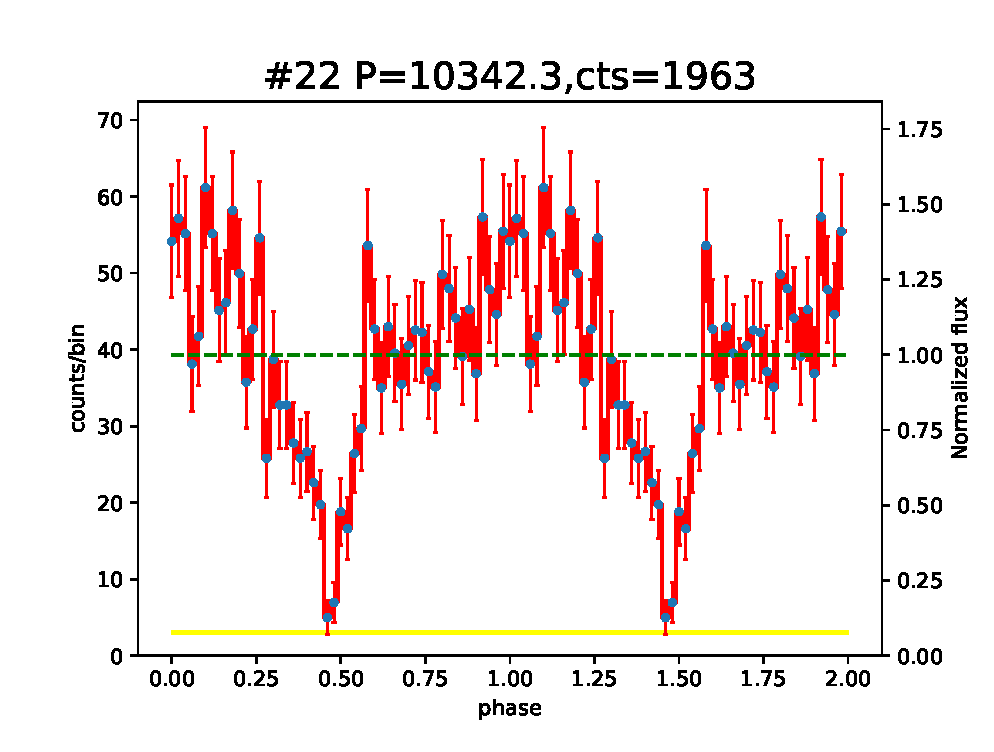
\includegraphics[width=\textwidth]{./figure/LW/pfold_lc_153002.eps}
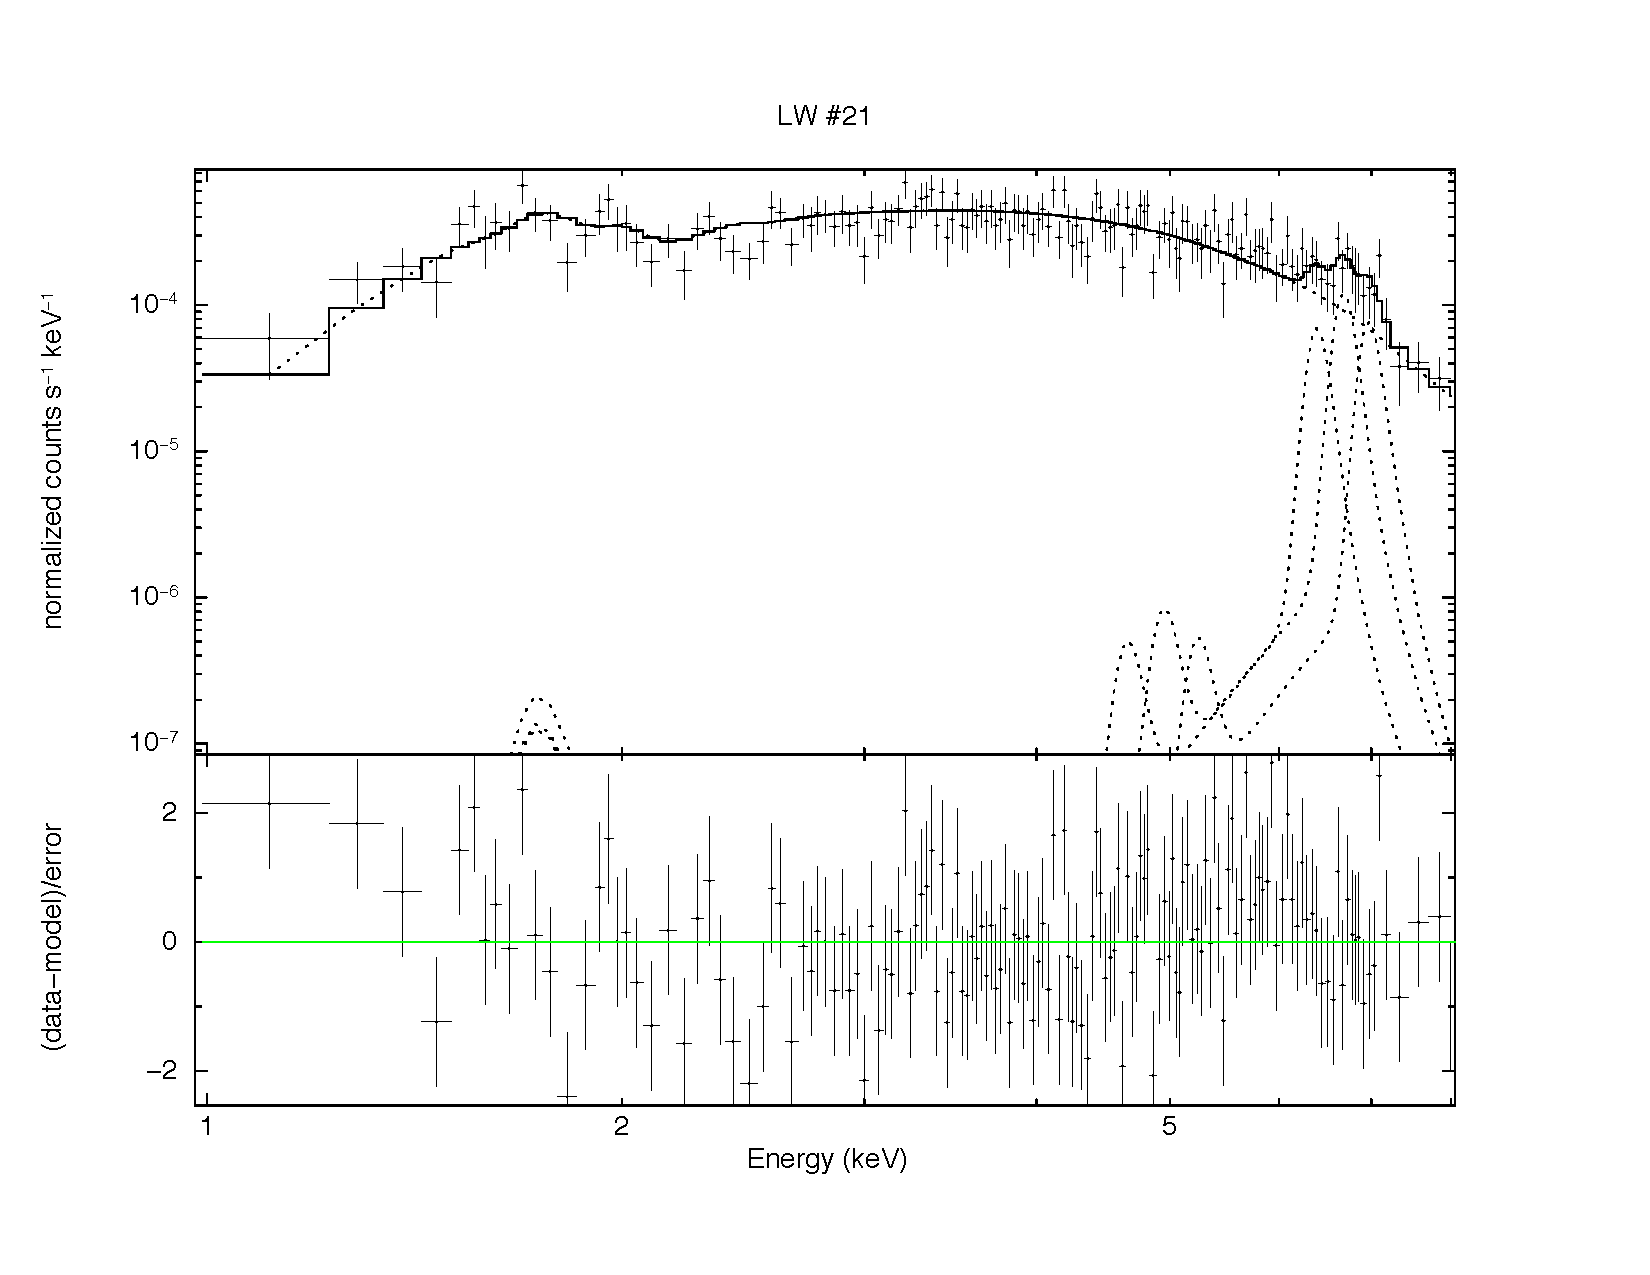
\includegraphics[width=1.02\textwidth]{./figure/LW/153001_spec.pdf}
\end{minipage}
\caption{Similar to Figure~\ref{fig:pCV_sample_1}, but for source \#21/\#22.}
\label{fig:pCV_sample_2}
\end{figure*}

\section{X-ray spectral analysis}\label{sec:spectra}
We perform spectral analysis for all 23 confirmed periodic sources to gain insight on their nature. Source and background spectra are extracted from the same regions as described in Section~\ref{subsec:detect}, along with the ancillary response files (ARFs) and redistribution matrix files (RMFs), by using the CIAO tool \emph{specextract}. 
The spectra from individual observations are then coadded to form a combined spectrum of a given source, with the corresponding ARFs and RMFs weighted by the effective exposure. 
Further, the spectrum is adaptively binned to achieve a minimum of 20 counts and a signal-to-noise ratio greater than 2 per bin.
The resultant spectra are analyzed using XSPEC v12.9.1.

%The reason we present the fitting results of 0.5-8 keV here is to constrain the absorption. Notice that the choice of energy range is not consistent with the illustration of spectra in Figure \ref{fig:Figure_p}, even though it has little impact on exhibition. 
Since these sources are expected to be CVs, we adopt a fiducial spectral model, which consists of a bremsstrahlung continuum and three Fe lines \citep{2018ApJS..235...26Z,2019ApJ...882..164X}. 
%three Gaussian lines centered at , 
We model each line with a Gaussian profile, fixing their line centroid at 6.40, 6.68 and 6.97 keV, respectively, and adopting a zero line width. 
All model components are subject to an unknown line-of-sight absorption (\emph{phabs} in XSPEC). 

It turns out that the plasma temperature ($T_{\rm b}$) is not well constrained in most sources, due to a moderate number of counts and the insufficient sensitivity of {\it Chandra} at energies above 8 keV. Hence for such cases we fix $T_{\rm b}$ at 40 keV, which is typical of IPs when their hard X-ray (up to tens of keV) spectra are available \citep{2016ApJ...818..136X,2016ApJ...826..160H}.
Setting a lower value of $T_{\rm b}$, for instance, at 20 keV, does not affect our following conclusions. 

Physically, the three lines (hereafter referred to as the 6.4, 6.7 and 7.0 keV lines) correspond to neutral Fe K$\alpha$, Fe\,XXV K$\alpha$ and Fe\,XXVI Ly$\alpha$, respectively, which are among the most commonly detected emission lines in CV spectra. The latter two lines, in particular, arise from the post-shock plasma near the WD surface, and their flux ratio ($I_{7.0}/I_{6.7}$) has proven to be a robust tracer of the plasma temperature, hence also a good indicator of the WD mass \citep{2016ApJ...818..136X}.
Unfortunately, again due to the limited number of counts, the Fe lines are absent or weak in most of the 23 sources.
We have applied a bootstrapping method using the {\it multifake} tool in XSPEC to derive the confidence range for the fluxes of the three Fe lines. Only one sources, \#21 (same as \#22), shows a significant ($\geq 3 \sigma$) line at both 6.7 keV and 7.0 keV. 
The flux ratio is $I_{7.0}/I_{6.7} = 0.91^{+1.22}_{-0.56}$ (90\% errors). Three additional sources (\#2, \#20 and \#23) show a significant 6.7 keV only.   


%The flux ratio of Fe XXVI to Fe XXV emission lines (hereafter $I_{7.0}/I_{6.7}$) could be interrelated to the $M_{WD}$ by uniting the $I_{7.0}/I_{6.7}$-$T_{max}$ and $T_{max}-M_{WD}$ relations \citep{2019ApJ...882..164X}. 

%The value of flux ratios are presented together with their 68.3\% confidence range (see column (4) and (5) in Table \ref{tab:spec}). 

%According to the empirical line ratio--WD mass  ($I_{7.0}/I_{6.7}$--$M_{\rm WD}$) relation of \citet{2019ApJ...882..164X}, which is calibrated with CVs in the solar neighborhood, we can infer $M_{\rm WD} \approx 0.8 \, (1.2) $  $M_\odot$ for \#21, provided that both sources are IPs (DNe). 
%It is noteworthy that there exists no empirical $I_{7.0}/I_{6.7}$--$M_{\rm WD}$ relation for polars, mainly due to the small number of known polars in the solar neighborhood \citep{2019ApJ...882..164X}. 

%We further  the 23 periodic sources into two groups based on their luminosities. The H (L) group consists of 6 (17) sources having an unabsorbed 1--8 keV luminosity above (below) $\rm 1.0\times10^{32}~erg ~s^{-1}$, which is derived from the individual best-fit spectral model. 
%The cumulative spectrum of each group is fitted with the same fiducial model, i.e., bremsstrahlung plus three Gaussian lines. The improved S/N in the cumulative spectrum allows us to detect all three Fe lines and constrain their flux ratios.  
%And the best-fit results are presented in Table \ref{tab:spec}. 
%The H and L spectra are shown in Figure \ref{fig:pCV_spec} over the energy range of 0.5-8 keV. 
%Using the XSPEC tool \emph{multifake}, we have gotten well constrained line ratios for this two subtypes. 
%The group has $I_{7.0}/I_{6.7} = 0.78^{+0.18}_{-0.16}$, thus inferring a mean WD mass of $M_{\rm WD} \approx 0.8$ (1.2) $M_\odot$ if they are IPs (DNe). 
%On the other hand, the L group shows no constrain of line ratio, we can only provide its upper limit, i.e., 0.39, corresponding $M_{\rm WD} < 0.45$ (0.80) $M_\odot$ if they are IPs (DNe). 
%We further generate an aggregated spectrum for all sources without a significant Fe 6.7 keV line. 
%the exception of \#21(22) and \#25, since the former may dominate the iron line emission and the latter is classified as an AB (see in Section \ref{subsec:class}).
%This group has $I_{7.0}/I_{6.7} \sim 0.19$, 
%thus inferring a mean WD mass of $M_{\rm WD} \approx ?$ (?) $M_\odot$ if they are IPs (DNe).

Results of the above spectral analysis are summarized in Table \ref{tab:spec}. We have also derived the 1--8 keV unabsorbed luminosity based on the best-fit model. 
It is noteworthy that source \#24 has an absorption column density of $0.35^{+0.16}_{-0.13}\times10^{21}{\rm~cm^{-2}}$, significantly lower than the expected column density of the LW, $N_{\rm H} \geq 7\times10^{21}{\rm~cm^{-2}}$ \citep{2011MNRAS.414..495R}. Hence 
this source may be located in the foreground, and its true luminosity can be substantially lower than that listed in Table \ref{tab:spec}. 

\begin{table*}
\centering
\begin{threeparttable}
\caption{X-ray spectral properties of the periodic sources \label{tab:spec}}
\begin{spacing}{1.19}

\begin{tabular}{lcccccc}
\hline
\hline
ID & $N_{\rm H}$ & $T_{\rm b}$ &  $EW_{6.7}$ &$I_{6.7}$ & $\chi^2$/d.o.f & $L_{\rm 1-8}$ 
\\
(1) & (2) & (3) & (4) & (5) & (6) & (7)
\\
LW & $10^{22}\rm~cm^{-2}$ & keV & keV & $\rm 10^{-8}~ph~ cm^{-2}~s^{-1} $ & & $10^{31}\rm~erg~s^{-1}$ 
\\
\hline

1$^\dag$ & $0.51^{+0.75}_{-0.34}$ & 40 (fixed)  & - & - & 0.72/8  & $2.02^{+0.71}_{-0.57}$
\\
2 & $2.17^{+0.54}_{-0.46}$ & $20.7^{+56.9}_{-9.92}$ & $0.63^{+1.17}_{-0.35}$ & $18.1^{+11.1}_{-9.32}$ & 0.86/78  & $25.7^{+3.00}_{-2.24}$
\\
3 & $1.38^{+0.39}_{-0.32}$ & 40 (fixed) & - & - & 0.98/35  & $7.34^{+1.17}_{-0.86}$
\\
4 & $1.15^{+0.69}_{-0.50}$ & $11.3^{+53.3}_{-4.71}$ & - & - & 0.91/27  & $25.0^{+3.27}_{-4.91}$
\\
5 & $1.02^{+0.27}_{-0.23}$ & 40 (fixed) & - & -& 1.00/35 &  $6.21^{+0.86}_{-0.78}$
\\
6 & $1.82^{+0.57}_{-0.50}$ & $6.90^{+12.4}_{-2.90}$ 
	& - & -& 1.12/42 &  $10.3^{+1.38}_{-1.23}$
\\
7 & $1.62^{+0.62}_{-0.49}$ & $41.6^{+43.0}_{-32.3}$ & - &- & 0.86/39 &  $7.45 ^{+0.99}_{-0.90}$
\\
8 & $2.06^{+1.51}_{-0.94}$ & 40 (fixed) & - &- & 0.93/7 &  $1.96^{+0.60}_{-0.47}$
\\
9 & $1.29^{+1.34}_{-0.67}$ & $20.8^{+95.8}_{-20.8}$ & -  &- & 1.10/7 &  $3.88^{+1.36}_{-0.96}$
\\
10 & $2.50^{+7.25}_{-1.56}$ & 40 (fixed)  & - &- & 0.85/5 &  $2.38^{+1.96}_{-0.84}$
\\
11 & $1.85^{+0.39}_{-0.33}$ & 40 (fixed)  & - &- & 1.22/47 &  $10.5^{+1.24}_{-1.14}$
\\
12 & $6.23^{+9.67}_{-3.66}$ & 40 (fixed) &-&-& 0.78/6 &  $8.42^{+6.40}_{-3.25}$
\\
13 & $0.90^{+0.30}_{-0.24}$ & 40 (fixed) & - &- & 1.15/38 &  $9.43^{+1.25}_{-1.16}$
\\
14$^\dag$ & $0.51^{+0.75}_{-0.34}$ & 40 (fixed) & - &- &  1.14/5 &  $2.02^{+0.71}_{-0.57}$
\\
15 & $1.46^{+0.48}_{-0.38}$ & 40 (fixed) & - &- &  1.16/42 & $14.3^{+1.97}_{-1.79}$
\\
16 & $0.89^{+0.18}_{-0.16}$ & 40 (fixed) & - &-&  1.43/51  & $9.41^{+0.98}_{-0.92}$
\\
17 & $2.68^{+0.63}_{-0.52}$ & 40 (fixed)  & - &-&  0.75/36 & $12.5^{+1.78}_{-1.61}$
\\
18 & $2.01^{+0.92}_{-0.66}$ & 40 (fixed)  & -&- &  0.53/14  & $4.68^{+0.99}_{-0.85}$
\\
19 & $1.82^{+0.10}_{-0.10}$ & 40 (fixed)  & - &- &  0.95/185  & $93.2^{+3.61}_{-3.51}$
\\
20 & $2.09^{+2.45}_{-1.16}$ & $4.04^{+28.2}_{-2.54}$ & - &$14.1^{+9.46}_{-8.04}$ & 1.04/12  & $5.99^{+2.01}_{-1.64}$
\\
21$^\ddag$ & $2.83^{+0.25}_{-0.23}$ & 40 (fixed)  & $0.56^{+0.20}_{-0.21}$& 
$32.1^{+15.6}_{-13.7}$ & 1.10/147  & $66.7^{+3.61}_{-3.47}$
\\
22$^\ddag$ & $2.83^{+0.25}_{-0.23}$ & 40 (fixed)  &  $0.56^{+0.20}_{-0.21}$ & $32.1^{+15.6}_{-13.7}$ & 1.10/147  & $66.7^{+3.61}_{-3.47}$
\\
23 & $1.83^{+0.44}_{-0.37}$ & 40 (fixed)  & $1.15^{+0.71}_{-0.63}$  & $12.9^{+8.03}_{-6.31}$ & 1.43/37  & $10.3^{+1.36}_{-1.25}$
\\
24 & $0.35^{+0.16}_{-0.13}$ & $4.78^{+3.55}_{-1.58}$ & - &-&  1.19/55  & 
$9.70^{+1.22}_{-1.09}$
\\
25 & $0.83^{+3.31}_{-0.83}$ & $2.30^{+1.59}_{-0.85}$ &-&-&  0.80/2 & $0.84^{+0.34}_{-0.31}$ 
\\
\hline
AG & $1.33^{+0.07}_{-0.07}$ & 40 (fixed) & $0.14^{+0.08}_{-0.08}$ &$2.12^{+1.23}_{-1.23}$& 1.04/204 & $11.8^{+0.32}_{-0.32}$\\
\hline
\end{tabular}
\end{spacing}
\begin{tablenotes}
      \small
      \item
      Notes: 
      (1) Source sequence number as in Table~\ref{tab:src}. {\dag}\#1 and \#14 are the same source with two different periods; {\ddag}\#21 and \#22 are the same source with two different periods. ``AG'' denotes the aggregated spectrum of all periodic sources except \#21(22) and \#25. 
(2) Line-of-sight absorption column density.
(3) The bremsstrahlung temperature, in units of keV. Fixed at a value of 40 keV when the spectrum provides no signficant constraint to this parameter.
 (4) Equivalent width of  6.7 keV line.
 (5) Integrated flux of the 6.7 keV line.
 (6) $\chi^2$ and degree of freedom of the best-fit model.
 (7) 1--8 keV unabsorbed luminosity. Quoted errors are at the 90\% confidence level.
\end{tablenotes} 
\end{threeparttable}
\end{table*} 
 
%\end{deluxetable*}
%

%\begin{figure*}[!htbp]
%\centering
%\rotatebox[origin=c,x=11pt,y=146pt]{270}{\includegraphics[width = 0.6\textwidth]{./figure/LW/pCV_brem.eps}}
%\caption{Cumulative spectra with the best-fit model($phabs\times (bremsstrahlung+gaussian+gaussian+gaussian) $).
%The spectrum for H, L set of periodic sources are plotted in red and black respectively. %\label{fig:pCV_spec}}
%\end{figure*}

\section{Discussion}\label{sec:discussion}
In this section, we discuss the most significant implications of our results. We first provide a comparison between our work and \cite{2012ApJ...746..165H} (Section~\ref{subsec:compare}). Then, we try to classify the periodic sources based on their temporal and spectral properties, demonstrating that the majority of these sources are most likely magnetic CVs (Section~\ref{subsec:class}). Lastly, we assess the potential sub-populations of CVs in the Galactic bulge (Section~\ref{subsec:population}).

\subsection{Comparison with previous work} \label{subsec:compare}
We have detected 25 periodic signals from 23 sources in the LW (Table~\ref{tab:src}). 
Our detections fully recover the 10 periodic signals from 10 sources found by \cite{2012ApJ...746..165H}. 
As illustrated in the upper panel of Figure~\ref{fig:com}, the measured periods between the two methods agree with each other to within 0.7\% and show no systematic bias.
The remaining 15 periods are new detections. 
Since \cite{2012ApJ...746..165H} and this work have used the same set of {\it Chandra} observations, 
this difference must be owing to the different period searching methods employed.

\cite{2012ApJ...746..165H} employed the LS periodogram,
%extracted only the several nearby observations, all the observations were applied here for timing analysis. That difference was caused by the mechanisms of methods. 
which, as described in Section~\ref{subsec:GL}, handles the photometric light curve, while the GL algorithm processes the phase-folded light curve with tolerance for observing gaps. We have applied the LS periodogram to our data in essentially the same way as \cite{2012ApJ...746..165H} and confirmed that only those 10 periods found in their work can be detected by this method. 
The other 15 periods do not result in a significant detection in the LS periodogram, mainly due to its low efficiency with low-count sources.
The detection rate is essentially zero for net counts $\lesssim$100 and never exceeds 20\% for net counts of 150, according to the simulations presented in \citet[figure 7 therein]{2012ApJ...746..165H}.

For comparison, we provide an estimate on the detection rate of the 10 commonly detected periodic signals using the GL algorithm. For practical purposes we assume an intrinsic sinusoidal shape (Eqn.~\ref{eqn:sin}), for which the total counts and period are taken directly from the observed values, whereas the relative amplitude ($A_0$) is taken 
%to be $A_{M}={1-R_{\rm min}}/R_{\rm max}$ and $A_{M}=2A_0/({1+A_0})$, where $R_{\rm min} (R_{\rm max})$ is the minimum (maximum) count rate of the folded light curve.
from \citet{2012ApJ...746..165H}, which was  based on the Rayleigh statistics \citep{1983A&A...128..245B,2003ApJ...599..465M}. 
%The definition of $A_{\mathrm{rms}}$ and the relation between 
%$A_{\mathrm{rms}}$ and $A_0$, which were taken by \cite{2012ApJ...746..165H}, are described below.
%\begin{subequations}
%\begin{equation}
%A_{\mathrm{rms}}=\left(\frac{Z_{1}^{2}}{N}\right)^{1 / 2} \frac{N}{N-B}
%\end{equation}
%\begin{equation}
%Z_{1}^{2}=\frac{2}{N}\left\{\left[\Sigma_{j} \cos \phi\left(t_{j}\right)\right]^{2}+\left[\Sigma_{j} \sin ^{2} \phi\left(t_{j}\right)\right]^{2}\right\}
%\end{equation}
%\begin{equation}\label{Arms}
%A_0=\sqrt{2} A_{\mathrm{rms}}
%\end{equation}
%\end{subequations}
%where equation \ref{Arms} only works for sinusoidal modulations. N and B represent the total counts in source region and local background respectively. $t_{j}$ and $\phi\left(t_{j}\right)$ refer to the arrival time and phase of each photon. $Z_{1}^{2}$ is the classical Rayleigh statistic method \citep{1983A&A...128..245B,2003ApJ...599..465M}.
%Though $A_{M}$ depends on the bin size of phase-folded light curve, we still prefer it rather than $A_{rms}$ to get the amplitude, i.e, $A_0$, since the deviation between sinusoidal variation and real shape sometimes made $A_{0}$ exceeds one when it was calculated from $A_{\mathrm{rms}}$. $A_{M}$ is obtained with bin size fixed at 20.
For each of the 10 signals, 100 simulated light curves are produced and fed to the GL algorithm.
Again, we take the 90\% probability threshold and a period accuracy of 1\% to define a valid detection. The percentage of valid detections, $P_{\rm det}$ (also listed in column 9 of Table~\ref{tab:src}), is plotted in the upper panel of Figure~\ref{fig:com}, along with the detection rate of the LS periodogram taken from \citet{2012ApJ...746..165H}.
%For directly comparison, we also ran the simulation based on the same $A_{0}$ defined in \citet{2012ApJ...746..165H} for the ten collective sources, the result of which is also plotted in Figure \ref{fig:com}.
Clearly, the GL algorithm works better in almost all cases compared to the LS periodogram. 

%The improvement on detecting efficiency and data usage brought more periodic signals than \cite{2012ApJ...746..165H}. Additionally, we operated the simulation not only for sinusoidal variation, but also for eclipsing models to describe the dip in orbital modulation. Combining the simulation results and more than twice the sample, we were allowed to discuss the source properties and the distribution of CVs in galactic bulge region on a better level.

\begin{figure*}
%\begin{minipage}[b]{\textwidth}
\centering
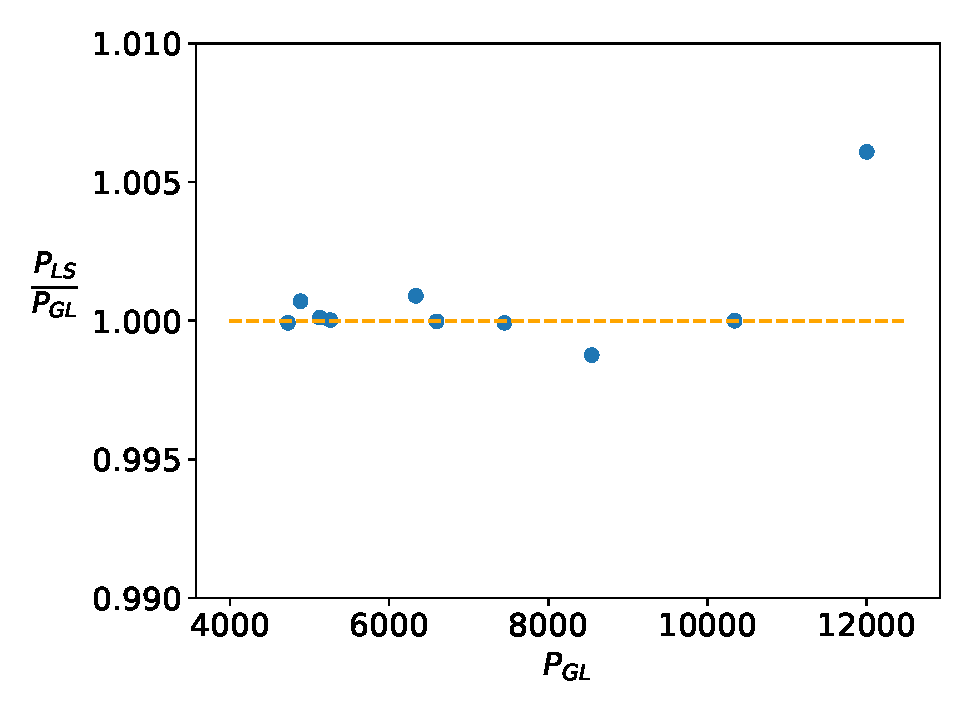
\includegraphics[width=0.49\textwidth]{./figure/LW/P_comp.eps}
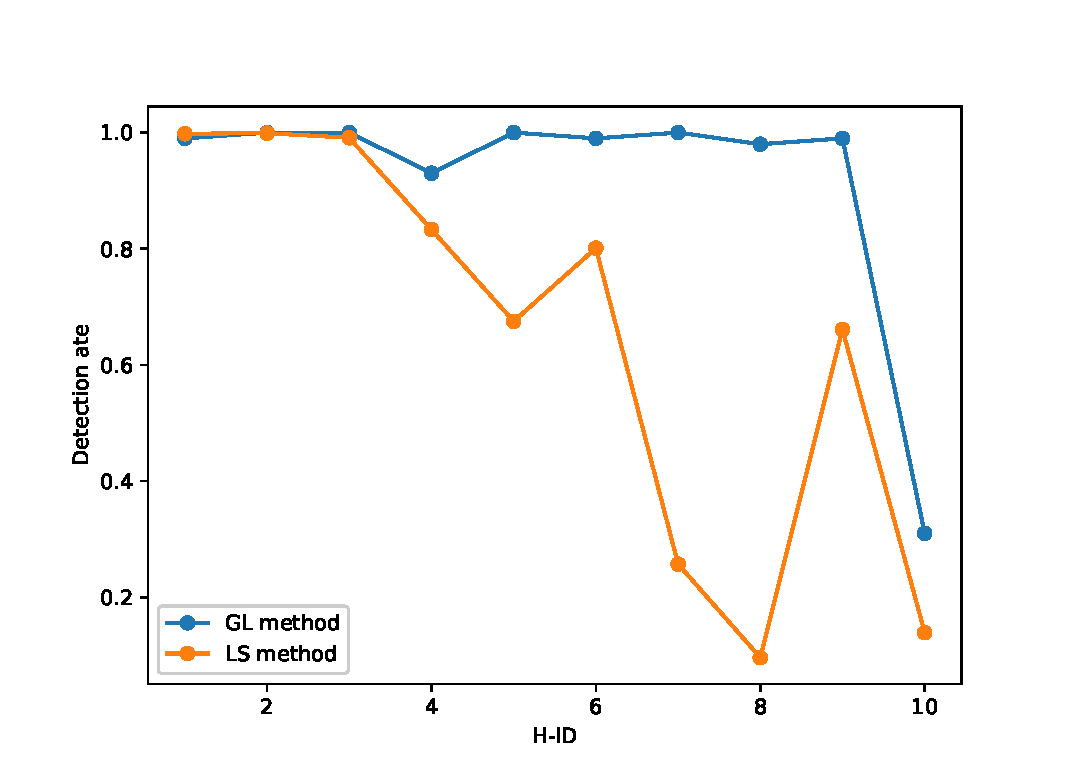
\includegraphics[width=0.46\textwidth]{./figure/sim_LW/Pdet_com.eps}
%\end{minipage}
\caption{Comparison between the period ({\it left}) and detection rate ({\it right}) of the 10 signals commonly found by the GL algorithm (this work) and the LS periodogram \citep{2012ApJ...746..165H}.The H-ID is the sequence number given in \citet{2012ApJ...746..165H}, same as listed in column 6 of Table \ref{tab:src}. 
\label{fig:com}}
\end{figure*}

\begin{figure*}
\centering
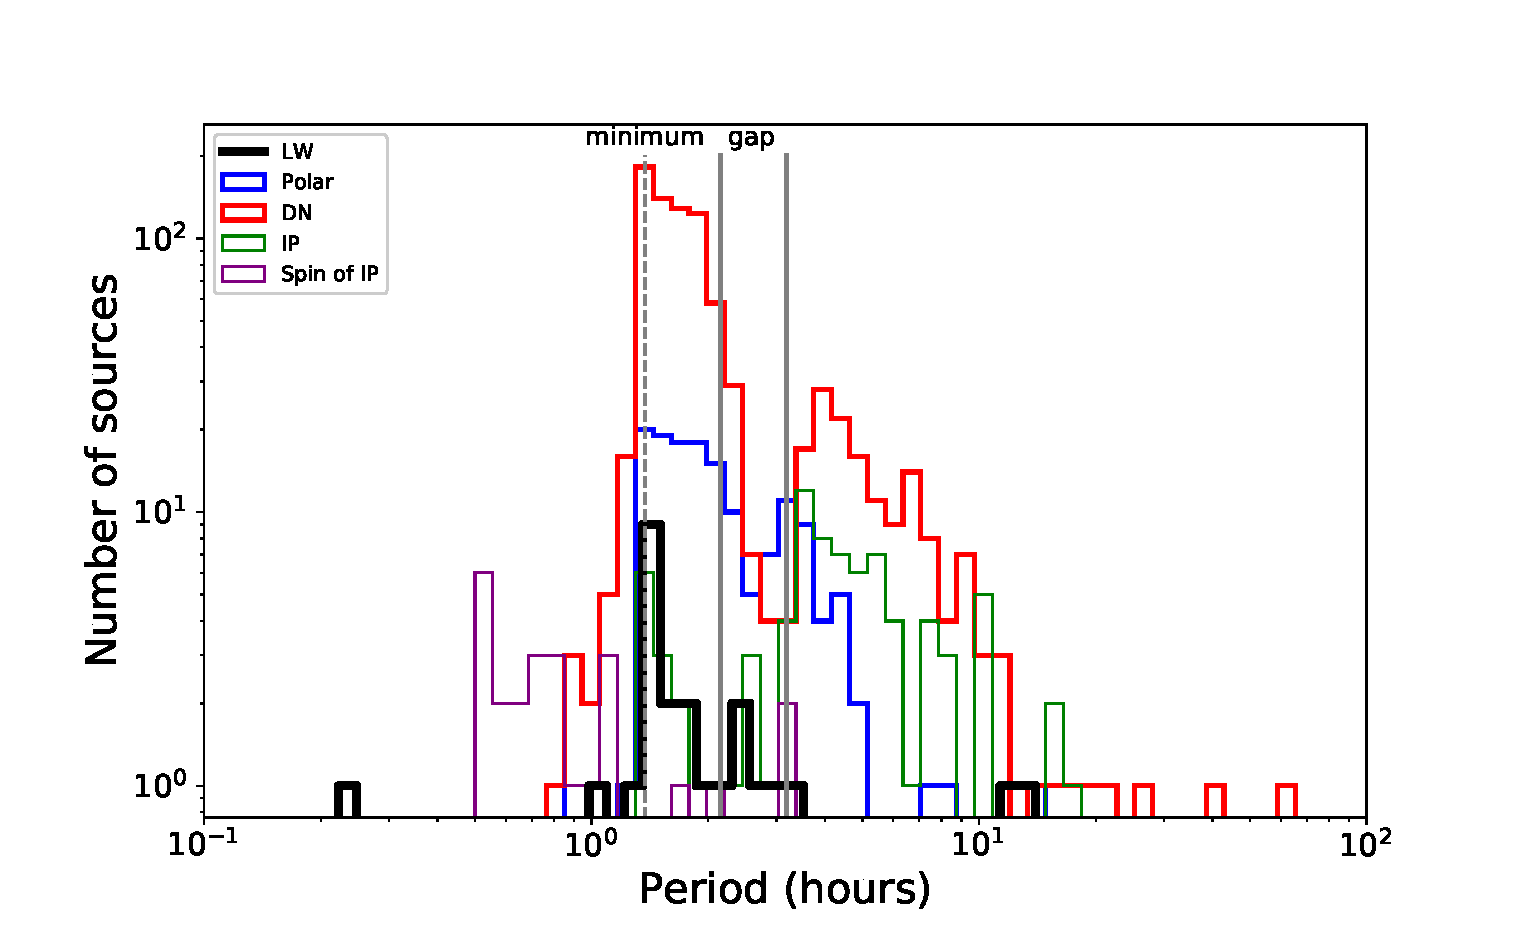
\includegraphics[scale=0.73]{./figure/CV/N_P.eps}
\caption{The period distribution of the LW sources (black histogram), in comparison with the spin (purple) and orbital (green) periods of IPs ,the orbital period of polars (blue), and the orbital period of DNe from the catalog of \citet{2003A&A...404..301R}, version 7.20. The period gap of CVs is delineated by a pair of vertical solid lines, and the period minimum is shown by a vertical dashed line, the values of which are taken from \citet{2011ApJS..194...28K}.\label{fig:N_P}}
\end{figure*}

\subsection{Classifying the periodic X-ray sources}
\label{subsec:class}
While it is generally difficult to unambiguously identify the nature of an X-ray source without knowing its optical counterpart, which is the case for most LW sources, the X-ray temporal and spectral properties of the 23 periodic sources contain useful information that actually allow for a reasonable classification for many of them. 

First of all, all but one (\#25) of these sources are found in the 1--8 keV luminosity range of $10^{31}-10^{33}\rm~erg~s^{-1}$ (Table~\ref{tab:spec}), which is typical of CVs. 
On the contrary, coronally active binaries (ABs), which are thought to dominate the detected X-ray sources in the LW by number \citep{2009Natur.458.1142R}, generally have unabsorbed X-ray luminosities below $\rm 10^{31}~erg~s^{-1}$ \citep{2006A&A...450..117S}. 
This stems from the empirical fact that the coronal X-ray emission from low-mass stars saturates at $\sim$10$^{-3}$ of the bolometric luminosity \citep{2004A&ARv..12...71G}.
The X-ray spectra of these sources are less informative, since except in a few cases they lack the unambiguous sign of Fe lines due to the moderate S/N (Section~\ref{sec:spectra}), which otherwise would be another characteristic signature of CVs (e.g., \citealp{2016ApJ...818..136X}).
Nevertheless, most of these sources do show a very hard continuum that are again typical of CVs, although this could be partially owing to the fact that our parent source list is based on the 2--8 keV band (Section~\ref{subsec:detect}).
Furthermore, the vast majority of the detected periods fall between 1.1--3.3 hours, consistent with the range of short-period CVs in the solar neighborhood \citep{2003A&A...404..301R}, i.e., those having an orbital period between the so-called period minimum and the upper bound of the period gap, as illustrated in Figure~\ref{fig:N_P}. 
Therefore, the global X-ray properties point to CVs dominating the detected periodic sources, a conclusion also drawn by \cite{2012ApJ...746..165H}.

It will then be interesting to ask to which sub-class of CVs these periodic sources belong. The phase-folded light curves may provide useful hints to this question. 
In magnetic CVs, including polars and IPs, their orbital and spin modulations can give rise to a characteristic light curve. For polars, let us consider the simplistic situation in which hard X-rays (photon energy $\gtrsim$1 keV) are produced in only one of the two magnetic poles\footnote{In this picture, accretion can still take place in the other pole, in fact, at a much higher accretion rate, producing quasi-black-body emission peaking at the soft X-ray and extreme ultraviolet bands \citep{2001cvs..book.....H}.}.
%Then the shape of light curve would be divided into two groups.
Denoting $i$ the angle between the line-of-sight and the spin axis, $\beta$ the angle between the spin and magnetic axes, and $\epsilon$ the magnetic colatitude of the accretion column, when $i+\beta+\epsilon > 90^{\circ}$, the two poles will alternately drift across the front side of the WD. 
The resultant light curve will look like that of source \#6 , \#8 and \#10, with nearly half of the cycle showing a valley of near-zero hard X-ray flux \citep{1985A&A...148L..14H}. 
The periods of these sources are consistent with the period range of known polars (for polars the orbital and spin periods are equal; Figure~\ref{fig:N_P}).
This so-called ``two-pole'' behavior becomes more complicated if hard X-rays were produced near both poles, in which case the second pole can partially fill the ``valley'', resulting in a light curve like that of \#4, \#5, \#9, \#12, \#13, \#15 ,\#16, \#17, \#23 and \#24. 
%Sometimes it may completely reverse in hard X-ray band cause the accretion shock in second pole producing most of hard X-rays. 
On the other hand, if $i+\beta+\epsilon < 90^{\circ}$ and $\beta < i$, the hard X-ray-emitting pole would be always visible (so-called ``one-pole'' behavior), producing a roughly constant light curve, although at certain phase dips can still present due to obscuration by the accretion stream.

IPs share the above two-pole and one-pole behavior. 
In addition, the orbital modulation can result in obscuration by the companion star \citep{1993MNRAS.260..299H}, by the accretion stream, or by the ``disc overflow'' \citep{1996MNRAS.280..937N}. 
Thus the light curve shape of IPs is often complex and can exhibit both sinusoidal variations and dips. Examples of this kind are found in sources \#3, \#7, \#11, \#18 and \#20.
We also consider source \#19 is a likely IP, for it has both the highest X-ray luminosity ($9.3\times10^{32}{\rm~erg~s^{-1}}$) and lowest variation ($\sim$20\%) among all sources. Its sinusoidal-like variation is quite possibly due to orbital modulation.

The most robust identification of IPs is to detect both the spin and orbital periods. Among our sources, \#1 (\#14) and \#21 (\#22) show two different periods.
For \#1, the period is 853.8 sec and the corresponding phase-folded light curve is consistent with the one-pole behavior (Figures~\ref{fig:pCV_sample_1}). This is naturally understood in terms of a spin modulation. 
In the meantime, the phase-folded light curve of \#14 shows a dip at phase 0.9--0.1, which may be understood as obscuration by the accretion stream, i.e., an orbital modulation. The corresponding orbital period of 5608.2 sec is reasonable for IPs. 
The two periods of \#21 and \#22 differ by only 5\% from each other (9877.5 sec vs. 10342.3 sec).
The light curve of \#22 exhibits a prominent narrow dip near phase 0.5 (Figure~\ref{fig:pCV_sample_2}). This is a clear sign of eclipse when viewed from a high inclination, thus the period of \#22 should be the orbital period. 
On the other hand, the light curve of \#21 resembles the two-pole behavior and is best understood as due to spin modulation. 
%Considering that the angle between the magnetic and spin axes ($\beta$) is usually small, the moderate variation also makes sense.
In this regard, source \#21/\#22 is probably an IP or a so-called asynchronous polar. 

It is worth asking, if some of the aforementioned sources (\#3, \#7, \#11, \#18, \#19 and \#20) were indeed IPs, why only their orbital period is detected. One plausible explanation is that their spin period, presumably below $\sim$ 1 hour, escapes detection due to a relatively low detection efficiency. Our simulations (Section \ref{subsec:simulation}) suggest that for moderate total counts and moderate variation amplitude, the detection rate is generally low for short periods. This effect may apply in all those six candidate IPs except \#19, which has total counts of 3402. Perhaps this source has a very low spin modulation due to the ``one-pole'' behavior.
One the other hand, source \#2, which has not been discussed so far, shows a period of 3820.8 sec, significantly lower than the canonical orbital period minimum of $\sim$82 minutes, determined from observations \citep{2009MNRAS.397.2170G} and theoretical modelling \citep{2011ApJS..194...28K}. %but also below the theoretical period minimum of 65 minutes in the standard model \citep{1982ApJ...254..616R}. 
Thus this period is more likely to be the spin period.
In this regard, a spike-like feature in the phase-folded light curve of \#2 may be caused by a bright spot on the WD surface. 
The unseen orbital modulation may be due to a low inclination angle. 

In DNe (i.e., non-magnetic CVs), hard X-rays are produced in the boundary layer near the WD surface, in which case spin modulation is essentially absent and orbital modulation is also expected to be weak, unless the inclination angle is sufficiently large to allow for a total eclipse. Among the 25 periodic signals, no clear sign of total eclipse is seen except for the case of \#22. However, we have argued in the above that source \#21/\#22 is an IP because of its dual period. Therefore, we probably have not detected any DN among the periodic sources. This is consistent with the low to moderate detection rates for eclipse predicted by our simulations in Section~\ref{subsec:simulation}. 

Lastly, we remark on the possible non-CV source \#25. This source has an unabsorbed 1--8 keV luminosity of $\rm 8.4 \times 10^{30}~erg~s^{-1}$, the lowest among all 23 sources. Its X-ray spectra, characterized by a best-fit plasma temperature of 2.3 keV (notably with large uncertainties; Table~\ref{tab:spec}), is also the softest among all sources.
These values are more typical of ABs. 
Moreover, the phase-folded light curve of \#25 suggests that the X-ray flux drops to the background level for nearly half of the 47317-sec period (Figure~\ref{fig:Figure_p}). 
As mentioned in the above, this may be due to a polar producing hard X-rays from only one of its two poles.
However, we consider such a case rather unlikely, since the corresponding period is much larger than that of any previous known polars (Figure~\ref{fig:N_P}), which would imply for an exceptionally strong magnetic field in the WD. 
Alternatively and more likely, this can be explained by a total eclipse lasting for half cycle.
In this case, the eclipsed star cannot be a WD, because of the mismatch between the stellar radius (order $10^4$ km)
and the orbital separation (order $10^7$ km).
Rather, the eclipsed star is likely to have a size not much smaller than the orbital separation, suggesting an AB system viewed nearly edge-on.
However, the near-zero flux for half-cycle is unusual for ABs. One possibility is that this system consists of a Sun-like star and an A-star, the latter producing no significant X-rays due to a very weak surface magnetic field \citep{2004A&ARv..12...71G}. 
An orbital separation of 4 $R_\odot$ estimated from the period is compatible with such a system. 
%Then the orbit radius would be around 0.02 AU, taking $3M_\odot$ as the total mass.  

In summary, based on the X-ray properties of the periodic sources, in particular their phase-folded light curves, we identify 13 candidate polars, 2 probable plus 7 candidate IPs, and one probable AB. 
Admittedly, polars and IPs share similar characteristics in their phase-folded light curves, as described above. The non-detection of the spin period (or orbital period in the case of \#2) brings about substantial uncertainty in the IP identification.
It is also noteworthy that only two long ($>3.5$ hours) periods are found among the 22 orbital periods (3 probable spin periods subtracted). This fraction ($\sim$9\%) is significantly smaller than the fraction of long-period magnetic CVs (IPs plus polars) in the solar neighborhood ($\sim$30\% according to the catalog of \citealp{2003A&A...404..301R}, version 7.20). 
This cannot be due to a selection effect of the GL algorithm, because our simulations in Section~\ref{subsec:simulation} predict that the detection rate is generally higher for longer periods.
\cite{2012ApJ...746..165H} noticed the narrow period distribution (1--3 hours) of the 10 sources they detected and the similarity with the period distribution of polars in the solar neighborhood (Figure~\ref{fig:N_P}), based on which they suggested that all these sources are polars. 
However, this could be due to an age effect, in the sense that CVs in the LW (bulge) are predominantly old and have substantially shrunk their orbitals, while CVs in the solar neighborhood can comprise of younger populations. 

\subsection{CV populations in the inner Galactic bulge}\label{subsec:population}
In the previous section, we have classified, with a varied degree of confidence, the 23 periodic sources, finding that the vast majority of them are either polars or IPs. Based on this classification, we now take one step forward to place constraints on the fraction of different sub-classes of CVs in the inner Galactic bulge, provided that the LW is a representative field.
%Before we start to discuss the nature of other periodic sources, we should take a look at CVs in the field. Their period distribution, including polars, IPs and DNe, are shown in Figure \ref{fig:N_P}.
%It can be easily seen that the period distribution of these LW sources resembles those of polars more than others, since most of these are below the period gap. While DNe and IPs both have a considerable number of systems with period beyond the gap.

The observed number of a given sub-class, for instance, polars, can be expressed as,
\begin{equation}
  N_{\rm det,polar} = P_{\rm det} \times g \times \alpha_{\rm polar} \times N_{\rm tot},
\end{equation}
where $N_{\rm tot}$ is the total number of CVs in the LW, $\alpha_{\rm polar}$ is the intrinsic fraction of polars among all CVs, $g$ is a geometric factor that determines the detectability of a periodic signal due to spin/orbital modulations, and $P_{\rm det}$ is the detection probability due to the GL algorithm. Here we take $N_{\rm tot}$ = 667, making the reasonable assumption that all LW sources with 1--8 keV total counts great than 100 are CVs and that CVs with a similar or larger total counts have been detected in 100\% completeness. 
%Firstly, we assumed that the fraction of polars in the total sample of 667 sources is $\alpha$ and 

We further assume that the substantial sinusoidal variation occurs only in the ``two-pole'' situation, that is, only one pole produces the hard X-rays and for this pole $i+\beta+\epsilon > 90^{\circ}$. 
Adopting an 50\% probability to fulfill each of these two conditions, this allows us to take $g_{\rm polar}$ = $50\%\times50\% = 25\%$ as the lower limit. In reality, $P_{\rm det}$ depends on the period, variation amplitude and total counts (Section~\ref{subsec:simulation}). We make use of our simulation results to estimate $P_{\rm det}$ with the following approximations:
(i) The short and long orbital periods (below or above 3 hours) are represented by $P$=5540 sec and $P$=45540 sec, respectively. A weight of 60\% (40\%) is assigned to the short (long) period, roughly according to the distribution of solar neighborhood polars; (ii) the amplitude is evenly sampled between 0.5 to 0.9, neglecting the contribution from any lower amplitudes (i.e., $P_{\rm det} = 0$ in this case);
(iii) the observed sources are grouped into different bins of total counts, from $C$=75 to 3575 cts at a step of 100 cts.  
%Then we obtain the mean detection rate from simulation, by combining the even distribution for amplitude from 0.5 to 0.9 and the harmonic average for results of P=5540s (60\%) and P=45540s (40\%). The value of 60\% and 40\% are estimated from the period distribution beyond and below the gap, respectively. Thus far, we get the detection rate only depended on number of counts.
%We set width=100 for our binning of counts, from 75 to 3575, covering nearly all detected sources. 
Then in each bin the number of polars is predicted to be
\begin{equation}
%Np_{i}=N_i\times DR \times 25\% \times \alpha	
N_{\rm det,polar}^i =  g_{\rm polar} \times \alpha_{\rm polar} \times P_{\rm det}^i \times N^i,
\end{equation}
where $N^i$ is the intrinsic number of sources in the bin, i.e., $\sum{N^i}=N_{\rm tot}=667$. 
%DR denotes the detection rate in this counts bin weighted from simulation. 
$N_{\rm det,polar}^i$ is constrained by the number of actually detected polars in a given bin. We take $\sum{N_{\rm det,polar}^i} = 20$, effectively counting all the periodic sources except the two probable IPs and the one probable AB (Section~\ref{subsec:class}).
%Then we sum all $Np_{i}$ together and force it equals to 20, getting $\alpha$ about 17\%. The value of 20 is taken as the upper limit by considering all periodic sources but three with determined properties (two IPs and one AB).
Figure~\ref{fig:NP_sim} compares the number of detected and predicted polars as a function of total counts, which apparently agree well with each other.  
This then requires $\alpha_{\rm polar} \approx 17\%$. Strictly speaking, this value is an upper limit, since a good fraction of the 20 periodic sources could be IPs and $g_{\rm polar}$ can also be higher than 25\%. 
For comparison, the fraction of polars is ??\% among all known CVs in the solar neighborhood as cataloged by \citet{2003A&A...404..301R}.

\begin{figure}
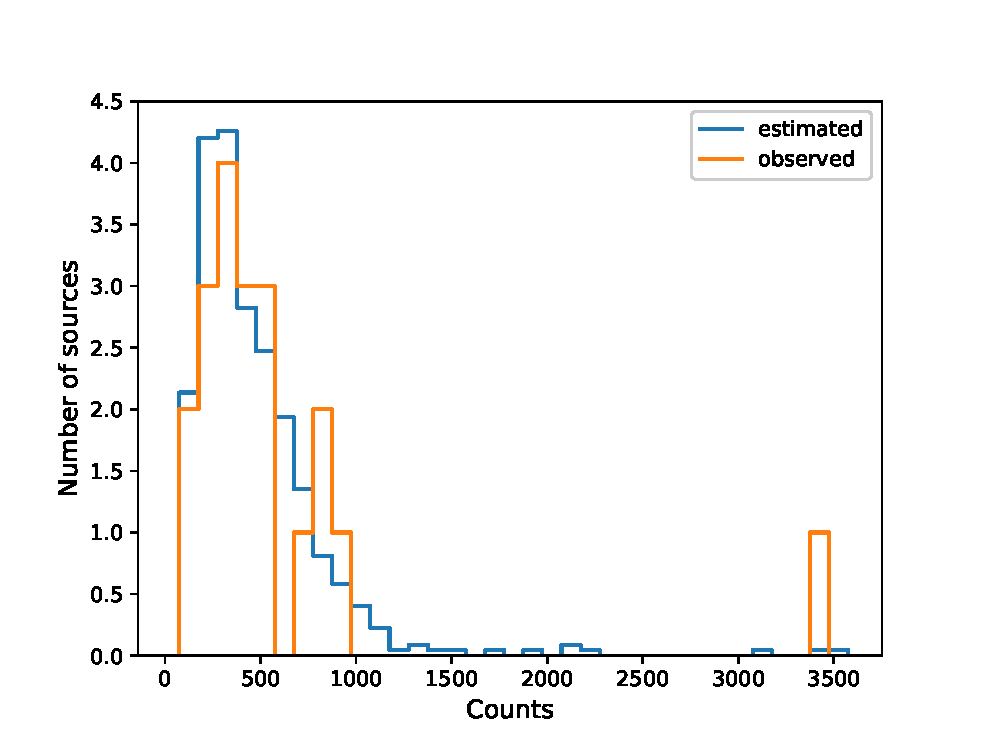
\includegraphics[scale=0.53]{./figure/sim_LW/est_obs.eps}
\caption{The comparison between the number of predicted and actually detected polars, as a function of detected counts number of sources. \label{fig:NP_sim}}
\end{figure}

%Since the real luminosity function should be gentle than that of total sample, which means there could be more polars at the bright band, then it demanding lower numbers of polar to balance the high detection rate for bright sources. Besides, with the intrinsic fraction (25\% as the lower limit) increasing, the $\alpha$ decreasing.
%In general, the 17\% should be treated as the upper limit for polars, especially when we considered all the 20 sources are polars. 

A similar approach can be applied to constrain the fraction of IPs, by evaluating the detectability of spin modulation. 
We still adopt $g_{\rm IP} = 25\%$ as the lower limit for detectable two-pole variation. The detected rate of the GL algorithm is represented by our simulations having a test period of $P=554$ sec. In Section~\ref{subsec:class}, we secure three periods as the spin period of IPs (\#1, \#2 and \#21). 
Hence, according to their total counts, we estimate the fraction of IPs to be 5\% in the LW. 
This is to be contrasted with ??\% in the solar neighborhood  \citep{2003A&A...404..301R}.

While for DNe, we are constrained by lack of reliable X-ray luminosity function(XLF). We could set one as the upper limit of DNe since no reliable detections of DNe. However, the steeper XLF for DNe than the XLF for total sample would only contribute the lower limit for their proportion. Though this conflict leads to the uncertainty of estimation,  we still present the estimation for fraction of DNe as supplement.
Intrinsically, the eclipse of white dwarf depends on the inclination angle, radius of companion star and orbit. If we set $i$ as inclination, $R_1$,$R_2$, $a$ as radius of WD, companion star and separation respectively. then eclipsing happens when :
\begin{equation}
{a \times cosi}\leq { R_1+R_2}
\end{equation}
Assuming that inclination angle is even distributed in $(0,90^\circ)$, the probability of eclipsing(hereafter EP) are plotted in Figure \ref{fig:simpCV}. The value of $R_1, R_2$ and $a$ are taken from simulation operated by \citep{2011ApJS..194...28K}, in which $R_1$ is fixed at when $M_{WD}$ equals 0.75 solar mass.
\begin{figure}
\centering
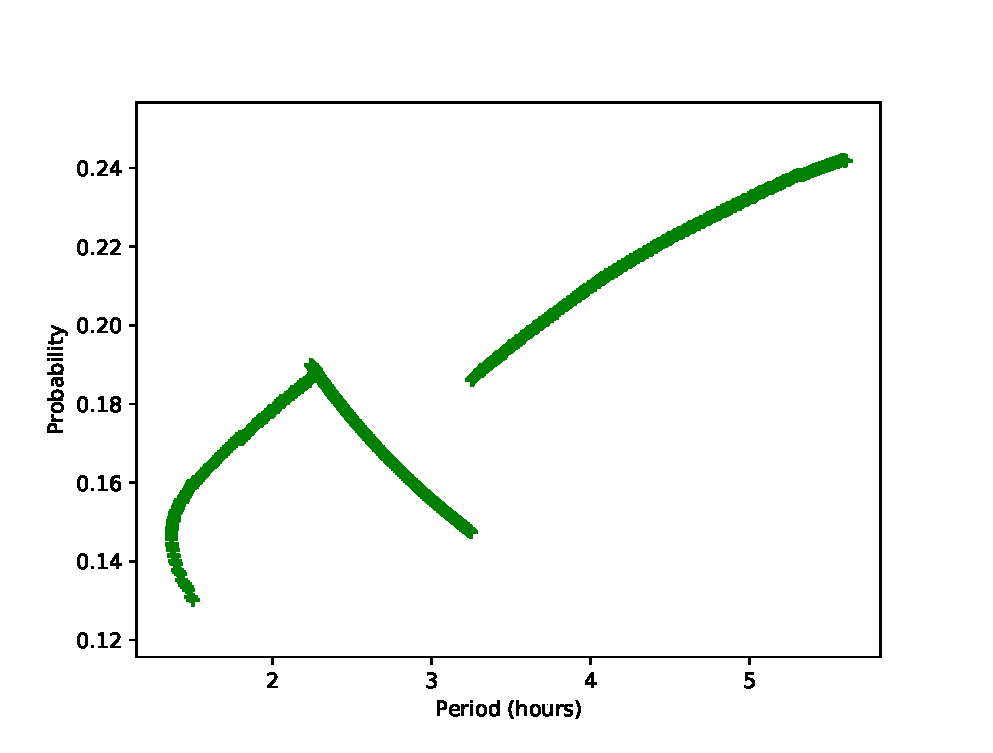
\includegraphics[scale=0.55]{./figure/p_inCV.eps}
\caption{Probability of eclipsing in CVs. The break around 3.2hours resulted by different model for CVs beyond and below the period gap.\label{fig:simpCV}}
\end{figure}

We utilized the simulation results of 5258s and 15258s as the detection rate for period under (75\% of the total number) and beyond (25\% of the total number) the period gap. The fraction is also taken from the statistics as shown in from Figure \ref{fig:N_P}. Besides, EP was chosen as 0.18 and 0.20 for this two types.
Similarly, the predicted number of periodic non-mCVs which "should" be detected in each counts bin is:
\begin{equation}
Np_{i}=N_i\times DR \times EP  \times \alpha	
\end{equation}
Since the sum of $Np_{i}$ was assigned as one, the $\alpha$ would be around 0.25 if we set $\rm 10^{32}~erg~s^{-1}$ (roughly corresponding 675 counts) as the upper limit of luminosity for DNe. The rationality of the limit has been proved by the DNe sample from solar neighborhood in \citep{2016ApJ...818..136X}, based on {\it Suzaku} observation. The uncertainty of this fraction comes from our limited acquaintance about XLF for DNe, and no detection of periodic DNe. 


\section{Summary}\label{sec:summary}

1. We have discovered 23 periodic sources with 25 signal in the LW by using GL method, including 10 of them already found by LS method in \cite{2012ApJ...746..165H}. Their luminosity range locates at $\rm 10^{31}-10^{33}~erg~s^{-1} $.The general feature of these 23 sources resembles that of polars. Two of them are determined as IP.

2.  We estimate the mass of WD from a source with great identification for Fe XXVI and Fe XXV emission lines, i.e. 0.8 $M_\odot$ for \#21(\#22) as being an IP. 

3. We provide well-constrained fraction of polars in the whole sample, i.e, 17\% as the upper limit. The estimation on fraction of non-mCVs is about 25\% while the certainty is restricted by limited appreciation about their XLF. Combined with the period distribution, we conclude that the periodic sources are mainly polars with relatively harder spectra, especially in the luminosity range that lower than $\rm 10^{32}~erg~s^{-1}$. Besides, the H sources (L>$\rm 10^{32}~erg~s^{-1}$), whose emission is mostly contributed by IPs, indicate  $M_{WD} \sim 0.8 M_\odot$, consistent with the previous result $0.8\pm 0.07 M_\odot$ in \citep{2018ApJ...853..182Y}.

4. The lower luminosity and narrow eclipsing model for orbital modulation reduced the detection rate simultaneously for periodicity. That may explain why we had no trace on non-mCVs in GCR in earlier period searching work.

5. We proved the higher detection rate, more usage of data and ignorance of observation gap for GL method compared with LS method. It is noteworthy that the shape of light curve in GL method could be modified according to different scenarios. It was applied on detection of planetary transits by using customized eclipsing model \citep{2002A&A...395..625A}. For the utility of GL method, there is still room for improvement in the future.
\\
\\

We thank Xiaojie Xu and Zhenlin Zhu for helpful discussions. This work is supported by the National Key Research and Development Program of China under grant 2017YFA0402703.

%% Appendix material should be preceded with a single \appendix command.
%% There should be a \section command for each appendix. Mark appendix
%% subsections with the same markup you use in the main body of the paper.

%% Each Appendix (indicated with \section) will be lettered A, B, C, etc.
%% The equation counter will reset when it encounters the \appendix
%% command and will number appendix equations (A1), (A2), etc. The

\bibliography{sample63}{}
\bibliographystyle{mnras}
%\onecolumn
\appendix
\section{A brief introduction to the Gregory-Loredo algorithm}\label{GL}
The basic rules for Bayesian probabilities are the sum rule,
\begin{equation}
p(H_i|I)+p(\bar{H_i}|I)	=1,
\end{equation}
and the product rule,
\begin{equation}\label{2.2}
p(H_i,D|I)=p(H_i|I)\cdot p(D|H_i,I)=p(D|I)\cdot p(H_i|D,I).
\end{equation}
From Eqn.~\ref{2.2} we can derive Bayes's theorem,
\begin{equation}\label{2.5} 
p(H_i|D,I)=p(H_i|I)\cdot {p(D|H_i,I)\over p(D|I)}.
\end{equation}
The symbols here follow \cite{1992ApJ...398..146G}.
Specifically, $p$ is the Bayesian posterior probability, $H_i$ denotes the $i$-th hypothesis, $D$ for the data, and $I$ for the ensemble of all hypotheses, i.e., all the model used.
The GL algorithm employs a stepwise function to detect periodic signal. Each model has $(m+2)$ parameters: the angular frequency $\omega={2\pi/P}$ ($P$ is the period), the phase parameter $\phi$, and $m$ values of $r_j$, which denotes the count rate in each phase bin where $j$=1 to $m$. In the following we replace $H_i$ by $M_i$ to denote the model where $i$ represents the number of bins in the stepwise model. Then the Bayes's theorem can be written as,
 \begin{equation}\label{2.11}
 p(M_i|D,I)=p(M_i|I)\cdot {p(D|M_i,I)\over p(D|I)}.
 \end{equation} 
We can write $I=M_1+M_2+M_3+\cdots$, where ``+'' stands for ``or''. Thus the proposition ($M_i$, $I$) is true if and only if model $M_i$ is true, i.e. ($M_i$, $I$) = $M_i$. The GL algorithm defines an odds ratio for model comparison,
\begin{equation}\label{2.12}
O_{ij}={p(M_i|D,I)\over p(M_j|D,I)}={p(M_i|I)\over p(M_j|I)}\cdot {p(D|M_i)\over p(D|M_j)}
\end{equation}
Note that $M_1$ means a constant model, $M_i$ ($i$=2,3,4...$N_{\rm mod}$, where $N_{\rm mod}$ is the total number of models considered) represents a periodic model. The probability for each model can be deduced from Eqn.~\ref{2.12},
\begin{equation}\label{6}
p(M_i|D,I)=O_{i1}\cdot p(M_1|D,I),
\end{equation}
thus
\begin{equation}\label{7}
p(M_1|D,I)={{\sum_{j=1}^{N_{\rm mod}} p(M_j|D,I)}\over {\sum_{j=1}^{N_{\rm mod}} O_{j1}}}
={1\over {\sum_{j=1}^{N_{\rm mod}} O_{j1}}}.
\end{equation}
Substituting Eqn.~\ref{7} into Eqn.~\ref{6}, we have
\begin{equation}\label{2.13}
p(M_i|D,I)={O_{i1}\over {\sum_{j=1}^{N_{\rm mod}} O_{j1}}}.
\end{equation}
Then the probability of a periodic signal is
\begin{equation}\label{5.2}
p(M_m(m>1)|D,I)={{\sum_{m=2}^{m_{\rm max}} O_{m1}}\over {1+\sum_{m=2}^{m_{\rm max}} O_{m1}}},
\end{equation}
where $m_{\rm max}$ is the maximum value of $m$.
The odds ratio can be calculated from the probability of the model,
\begin{equation}
O_{m1}={{p(M_m|D,I)}\over {p(M_1|D,I)}}.
\end{equation}
Using Bayes's theorem (Eqn.~\ref{2.11}), 
\begin{equation}\label{11}
O_{m1}={{p(M_m|I)\cdot p(D|M_m)}\over {p(M_1|I)\cdot p(D|M_1)}}.
\end{equation}
Following the assignment by \citet{1992ApJ...398..146G}, we assume that the periodic and aperiodic signals have the same probability. Then the priors for the models can be written explicitly as,
\begin{equation}\label{12}
p(M_1|I)={1\over 2},	
\end{equation}
\begin{equation}\label{13}
p(M_m|I)={1\over {2\nu}}, \quad \nu =m_{\rm max}-1.
\end{equation}

For astronomical data of Poisson distribution, it can be shown that (Equation 5.27 in \citealp{1992ApJ...398..146G}),
\begin{equation}\label{5.27}
\begin{split}
p(D|M_m)={{{\Delta t}^N (m-1)! N! \gamma(N+1,A_{\rm max})T}\over{2\pi A_{\rm max} (N+m-1)!T^{N+1} \ln(\omega_{\rm hi}/\omega_{\rm lo})}}\\
\times {\int_{\omega_{\rm lo}}^{\omega_{\rm hi}}}{{d\omega}\over{\omega}}\times {\int_0^{2\pi}d\phi{m^N\over W_m(\omega,\phi)}},	
\end{split}
\end{equation}
where $\omega_{\rm lo}$ and $\omega_{\rm hi}$ are the lower and upper bounds of the frequency range.
It should be emphasized that the above equation holds for the case in which the period and phase are both unknown.
Substituting $m=1$ into Eqn.~\ref{5.27}, we have
\begin{equation}\label{15}
p(D|M_1)={{{\Delta t}^N N!\gamma(N+1,A_{\rm max})T}\over {A_{\rm max}N!T^{N+1}}}.
\end{equation}
Substituting Eqns.~\ref{12}, \ref{13}, \ref{5.27} and \ref{15} into Eqn.~\ref{11}, the odds ratio can be written as follows, which is the same as Equation 5.28 in \cite{1992ApJ...398..146G},
\begin{equation}\label{A16}
\begin{split}
O_{m1}={1\over{2\pi \nu \ln(\omega_{\rm hi}/\omega_{\rm lo})}} {{N+m-1}	\choose N}^{-1}\times {\int_{\omega_{\rm lo}}^{\omega_{\rm hi}}}{{d\omega}\over{\omega}}\\
\times {\int_0^{2\pi}d\phi{m^N\over W_m(\omega,\phi)}} 
\end{split}
\end{equation}

Astronomical data are often subject to observational gaps. %For example, when the period is long and the exposure time for single observation is low, different bins may not be covered fairly. 
This may result in unevenly covered phase bins, leading to spurious detections especially at low frequencies. \cite{1992ApJ...398..146G} provides a solution to this problem, by introducing a weighting factor 
\begin{equation}\label{A17}
S(\omega,\phi)={\prod_{j=1}^m s_j^{-n_j}},
\end{equation}
\begin{equation}
s_j(\omega,\phi)={{\tau_{j}(\omega,\phi)}\over {T/m}},
\end{equation}
where $T$ is the total time span between the first and last photons and ${\tau_{j}(\omega,\phi)}$ denotes the exposure time in each phase bin.
Then the odds ratio should be modified as,
\begin{equation}\label{A19}
\begin{split}
O_{m1}={1\over{2\pi \nu \ln(\omega_{\rm hi}/\omega_{\rm lo})}} {{N+m-1}	\choose N}^{-1}\times {\int_{\omega_{\rm lo}}^{\omega_{\rm hi}}}{{d\omega}\over{\omega}}\\
\times {\int_0^{2\pi}d\phi{S(\omega,\phi)m^N\over W_m(\omega,\phi)}}.
\end{split} 
\end{equation}
Ultimately, the probability of whether the dataset is periodic is,
\begin{equation}\label{A20}
p({\rm periodic})={{\sum_{m=2}^{m_{\rm max}} O_{m1}}\over {1+\sum_{m=2}^{m_{\rm max}} O_{m1}}}.
\end{equation}
The posterior probability of the frequency contains the period of the signal,
\begin{equation}\label{A21}
O_{m1}(\omega)={1\over{2\pi \nu}} {{N+m-1}	\choose N}^{-1} \times {\int_0^{2\pi}d\phi{S(\omega,\phi)m^N\over W_m(\omega,\phi)}}.
\end{equation}
The period locates at $P=2\pi /\omega $ when $O_{m1}(\omega)$ takes the highest value.


%\section{Treatment of harmonics}\label{harmonics}
%
%\begin{figure*}
%\begin{minipage}[b]{0.45\textwidth}
%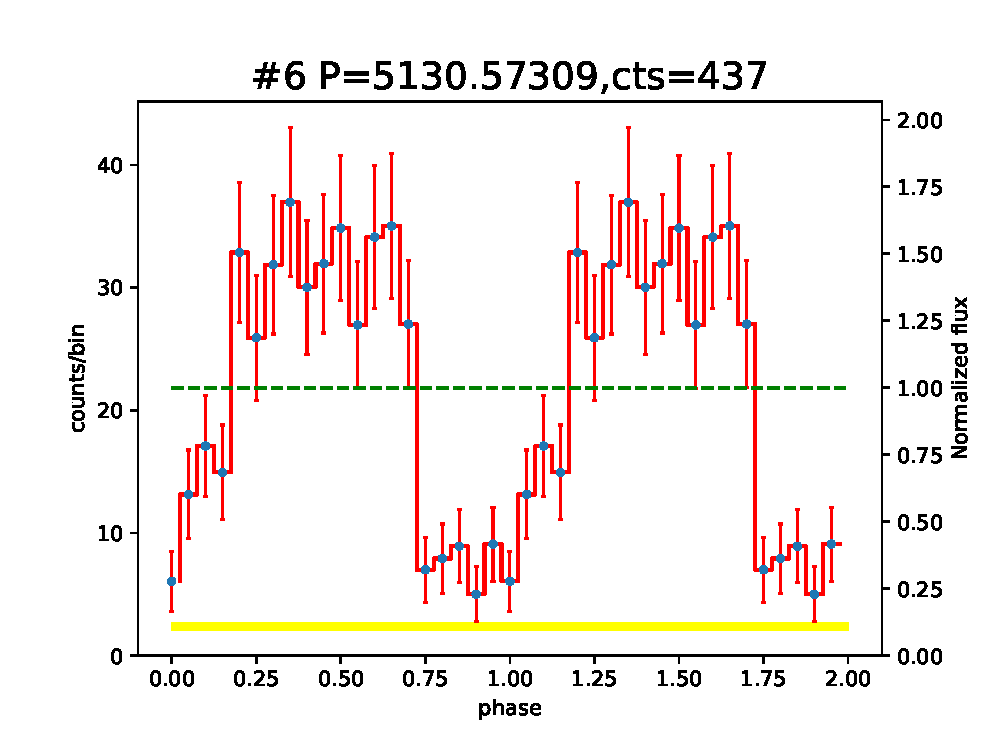
\includegraphics[width=\textwidth]{./figure/LW/pfold_lc_20.eps}
%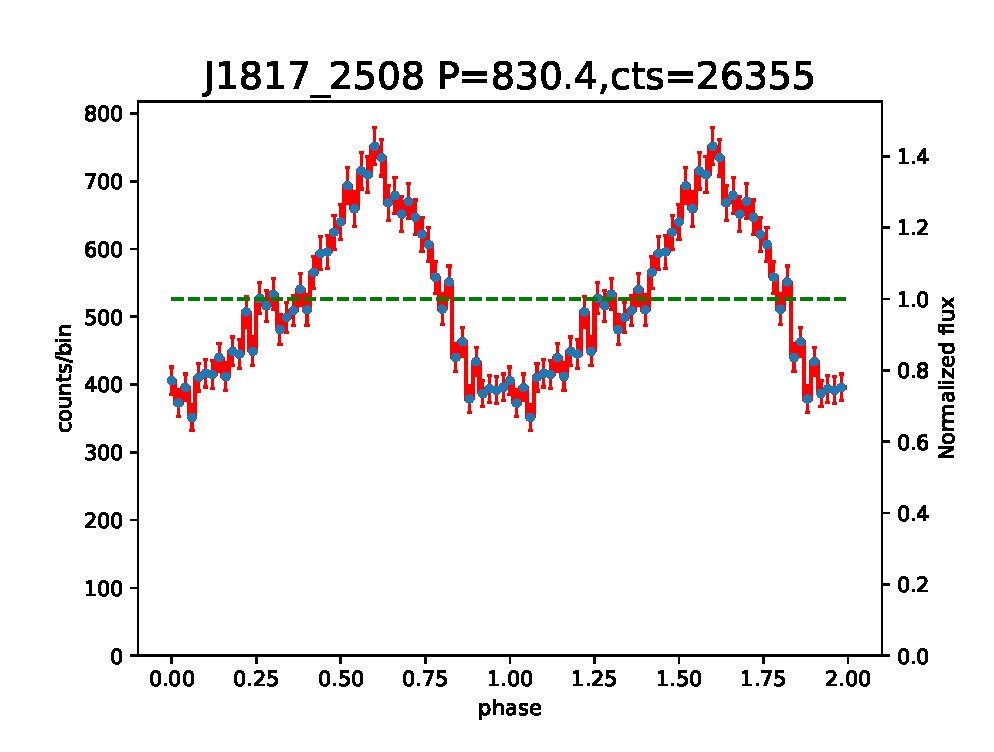
\includegraphics[width=\textwidth]{./figure/CV/pfold_lc_J1817_2508_spin_half.eps}
%\end{minipage}
%\begin{minipage}[b]{0.45\textwidth}
%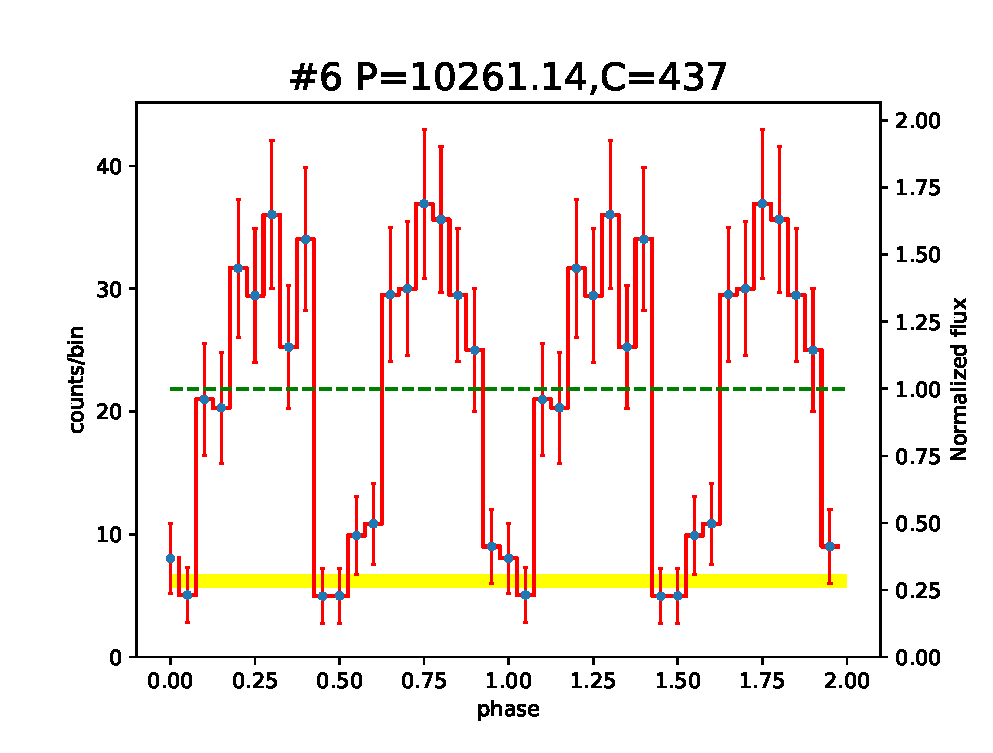
\includegraphics[width=\textwidth]{./figure/LW/pfold_lc_20_second.eps}
%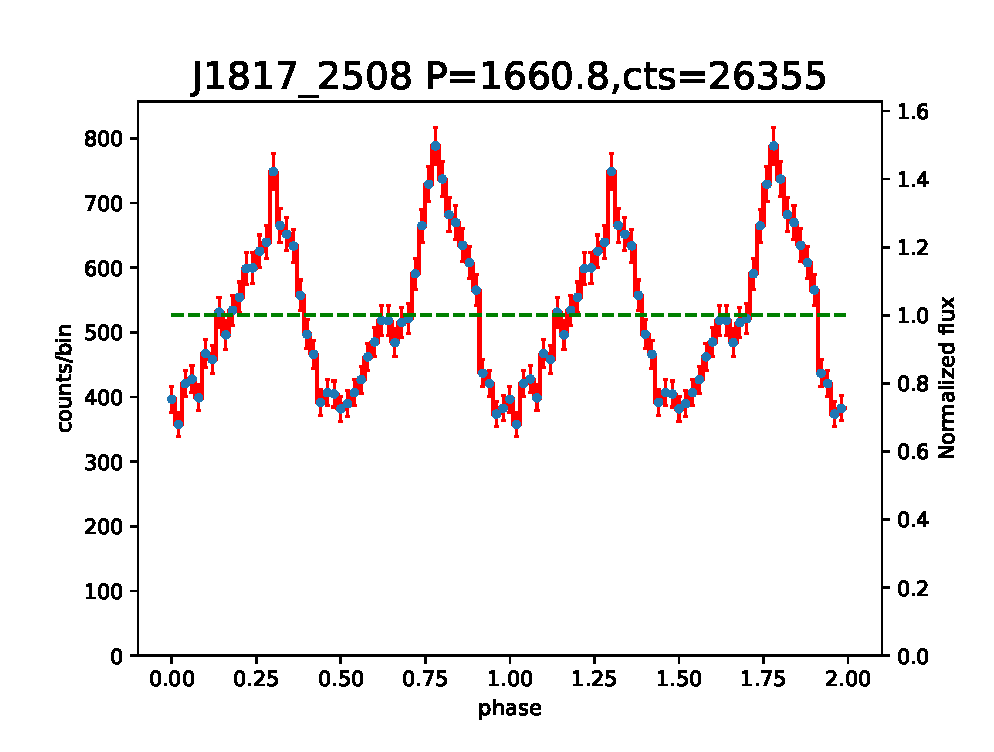
\includegraphics[width=\textwidth]{./figure/CV/pfold_lc_J1817_2508_spin.eps}
%\end{minipage}
%\caption{The top left and right panel show the folded light curve of LW 6, at true period and second harmonics, respectively. The lower left panel displays the folded light curve of J1817-2508. While for this source, the double-peaked shape (lower right) at 1660s are the real signal of rotation. \label{fig:6thfig}}
%\end{figure*}
%\indent
%To distinguish the fundamental period--whether it is the spin period or orbital period---from the harmonics, the significance of the signal is not the sufficient condition. 
%We have already assumed that no half harmonics in the LW sources (see \ref{subsec:simulation}) based on our simulation. This assumption can be  extra supported by physical origin of periodic signals in CVs.
%%In that the intensities of signals could not reflect the authenticity of the signal precisely.
%%Rather, the physical mechanism of period in CVs must be introduced. 
%Here we take source \#6 as an illustration. This source has two detected periods both exceeding the 90\% probability threshold. 
%The phase-folded light curves of the fundamental period and the second harmonics, plotted in the top panels of Figure \ref{fig:6thfig}, show a classical single-peak and double-peak shape, respectively. 
%If the half harmonics exists, the longer period has to serve as true signal. While theoretically, the double-peak shape generally only happens in IPs with an accretion column. When viewed from a specific angle, the two poles alternatively drift across the front side of the WD, producing the double-peaked shape in the X-ray light curve. In this kind of situation, the modulation period must be the spin period of IPs, typically under one hour, as illustrated in \ref{fig:N_P}.
%In our results, most of the double-peak shape light curves come up with period longer than 3 hour, far beyond the range of spin period in IPs. 
%For the above reasons, we preferentially take the single-peaked signal, normally due to the shortest period, as the true period. The second harmonics leading to a double-peaked shape is treated as a spurious period. 
%
%%As supplement for the theory , we present the phase-folded light curves of an IP called J1817-2508, who has the double-peak shape in rotational modulation (lower panels of Figure~\ref{fig:6thfig}), based on an {\it XMM-Newton} observation (obsID=0601270301) with an exposure of 32 ks.
%%We processed the EPIC/PN data with the standard tool \emph{emchain} and \emph{epchain} in SAS v18.0.0. The MOS data were neglected for simplicity.
%%The photon arrival times were corrected to the Solar barycenter by applying the task \emph{barycen}.
%%We then extracted the 0.2-10 keV counts of J1817-2508 from a circle of 25$\arcsec$).
%%
%%J1817-2508, also known as IGR J18173-2509, was first found to exhibit a periodic signal at 830.70 sec by {\it Swift}-XRT observations (reference?). An additional periodic signal of 1660 sec was detected by {\it Chandra} observations \citep{2009ATel.2354....1N}; a slightly larger period at 1690 sec was found by optical observations \citep{2012A&A...542A..22B}. 
%%Together these strongly suggest that the true spin period is about 1660 sec, twice the {\it Swift}-detected period, even though when folded at the second harmonics the light curve exhibits two highly similar peaks, as shown in the lower right panel of Figure~\ref{fig:6thfig}.
%% 
%%The case of J1817-2508 indicates that the phase-folded light curve itself could be highly deceptive under the circumstance of symmetric dipole structure. We cannot unambiguously determine the true spin period without additional information, e.g., from optical observations. 
%%
%%Fortunately, the physical origin of the periodic signal may provide help diagnostics.  The double-peak shape generally only happens in IPs with an accretion column. %The two poles where accretion region lied on, would be the brightest. 
%%When viewed from a specific angle, the two poles alternatively drift across the front side of the WD, producing the double-peaked shape in the X-ray light curve. In this kind of situation, the modulation period must be the spin period, typically under one hour. 
%%For comparison, the second harmonics found in the LW sources are mostly above 3 hours, thus they are unlikely to be the true spin period. 
%%On the other hand, while the WD in polars may have a spin period of few hours due to synchronization with the orbital period, their accretion stream always fall onto a single pole, emitting most of the X-rays. Thus the double-peaked shape is almost impossible in polars. 
% 
%%\clearpage
%%\newpage
\section{Additional figures of the periodic X-ray sources}\label{appen:fig}
  \begin{figure*}
    \centering
    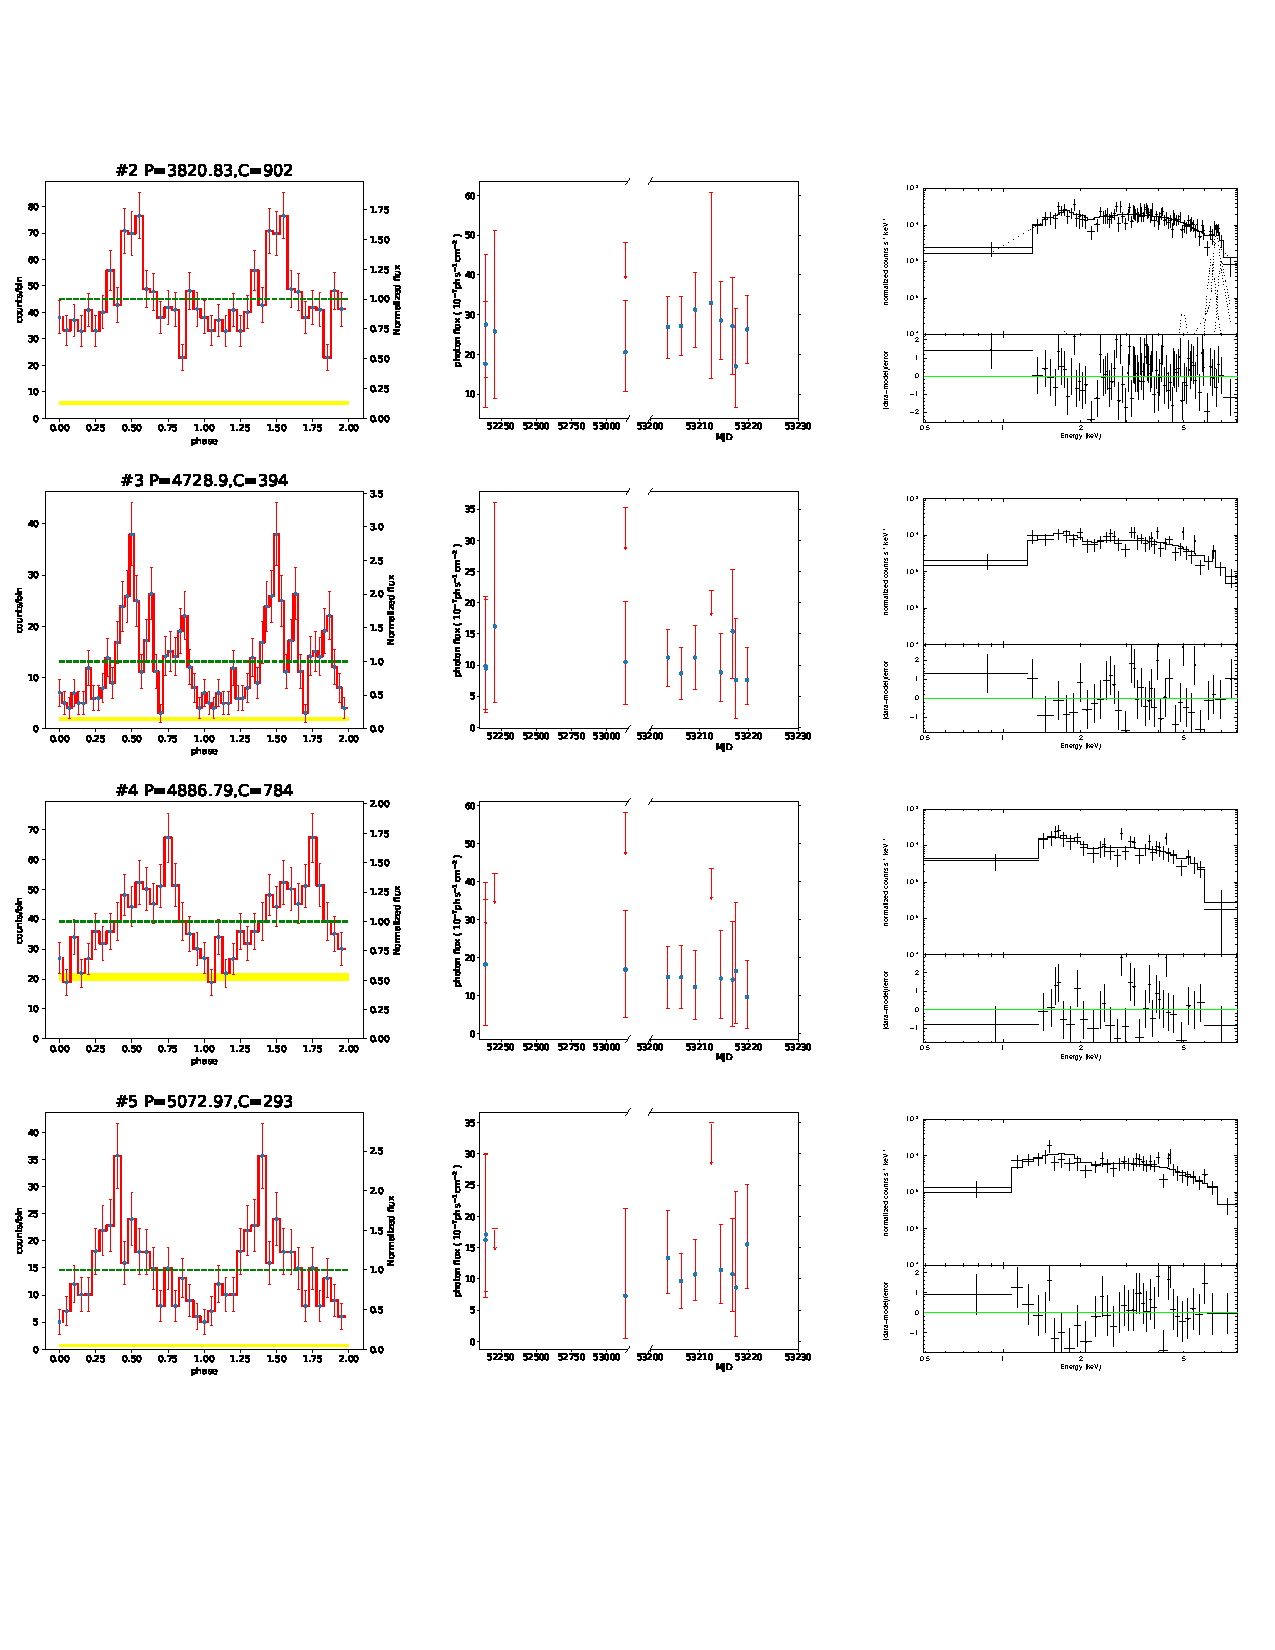
\includegraphics[page=1,scale=0.90,trim=0 100 0 20,clip]{plot_figure_LW.pdf}
    \caption{Each row shows one periodic source. {\it Left}: The 1--8 keV phase-folded light curve at the modulation period.
The green dashed line represents the mean count rate, whereas the yellow strip represents the local background, the width of which represents 1\,$\sigma$ Poisson error.
{\it Middle}: the 1--8 keV long-term, inter-observation light curve. Arrows represent 3\,$\sigma$ upper limits. 
{\it Right}: Source spectrum and the best-fit model. 
    \label{fig:Figure_p}}
  \end{figure*}
  
  \begin{figure*}
%    \ContinuedFloat
%    \captionsetup{list=off,format=cont}
    \centering
    \includegraphics[page=2,scale=0.90,trim=0 100 0 20,clip]{plot_figure_LW.pdf}
    \caption{Continued}
  \end{figure*}

  \begin{figure*}
%  \ContinuedFloat
%  \captionsetup{list=off,format=cont}
    \centering
    \includegraphics[page=3,scale=0.90,trim=0 100 0 20,clip]{plot_figure_LW.pdf}
    \caption{Continued}
  \end{figure*}
  
   \begin{figure*}
%  \ContinuedFloat
%  \captionsetup{list=off,format=cont}
    \centering
    \includegraphics[page=4,scale=0.90,trim=0 100 0 20,clip]{plot_figure_LW.pdf}
    \caption{Continued}
  \end{figure*}
  
  \begin{figure*}
%  \ContinuedFloat
%  \captionsetup{list=off,format=cont}
    \centering
    \includegraphics[page=5,scale=0.90,trim=0 100 0 20,clip]{plot_figure_LW.pdf}
    \caption{Continued}
  \end{figure*}
  
  \begin{figure*}
%  \ContinuedFloat
%  \captionsetup{list=off,format=cont}
    \centering
    \includegraphics[page=6,scale=0.90,trim=0 100 0 20,clip]{plot_figure_LW.pdf}
    \caption{Continued}
  \end{figure*}
  
%   \begin{figure*}
%%  \ContinuedFloat
%%  \captionsetup{list=off,format=cont}
%    \centering
%    \includegraphics[page=7,scale=0.90,trim=0 550 0 20,clip]{plot_figure_LW.pdf}
%    \caption{First figure continued}
%  \end{figure*}

%% For this sample we use BibTeX plus aasjournals.bst to generate the
%% the bibliography. The sample63.bib file was populated from ADS. To
%% get the citations to show in the compiled file do the following:
%%
%% pdflatex sample63.tex
%% bibtext sample63
%% pdflatex sample63.tex
%% pdflatex sample63.tex


\end{document}

% End of file `sample63.tex'.
